\documentclass{beamer}
\usetheme{dianahep}

%
% Title definitions
%

\title{The S2I2-HEP Conceptualization Project \\
       and the \\
       High Luminosity LHC at CERN}
\author{Peter Elmer - Princeton University} 
\date{1 May, 2017 \\ 2nd S2I2 HEP/CS Workshop}

\begin{document}
\maketitle
%\insertframenumber/\inserttotalframenumber

%
% Presentation body
%

\setbeamertemplate{footline}[frame number]

%\begin{frame}
\frametitle{2nd S2I2 Workshop on HEP and CS Collaboration}

Welcome to the 2nd workshop on collaboration between High Energy 
Physics (HEP) and Computer Science (CS).
\vskip 0.15in
The first S2I2 HEP/CS workshop was held at UIUC/NCSA in Dec., 2016, see
\url{https://indico.cern.ch/event/575443/}.
\vskip 0.15in
This is one of a number of workshops taking place this year through the summer as part of the conceptualization project for a possible NSF ``Scientific Software Innovation Institute'' (S2I2) focused on HEP (\url{http://s2i2-hep.org}).
\vskip 0.15in
We have a mix of returning and new attendees as this workshop. So after
some logistical/introductory material, I will describe the S2I2 HEP 
conceptualization project, the challenges motivating this project (and an eventual Software Institute) and the current status.
\vskip 0.15in

\end{frame}



%
%% Logistics
%
%\begin{frame}
\frametitle{Workshop venues}
See "Travel Information" on the workshop website (\url{https://indico.cern.ch/event/622920/}) for links to campus maps and iOS/Android apps for Princeton
\vskip 0.15in
\begin{itemize}
\item Monday (plenary) - Lewis Library 120 
\item Tuesday (parallel sessions) - Jadwin Hall A06,  Jadwin Hall 475, Jadwin Hall 111
\item Wednesday (plenary) - Lewis Library 138
\end{itemize}
Vidyo connections will be available on Monday and Wednesday for the plenary sessions.
\vskip 0.15in
On Monday/Wednesday the coffee breaks and lunch are outside the rooms in Lewis Library. On Tuesday coffee breaks, lunch and the posters will be in Brush Gallery (see map under "Travel Information"). This evening there will be a reception at Prospect House.
\end{frame}



%\begin{frame}
\frametitle{Workshop venues}

\begin{figure}[htbp]
\begin{center}
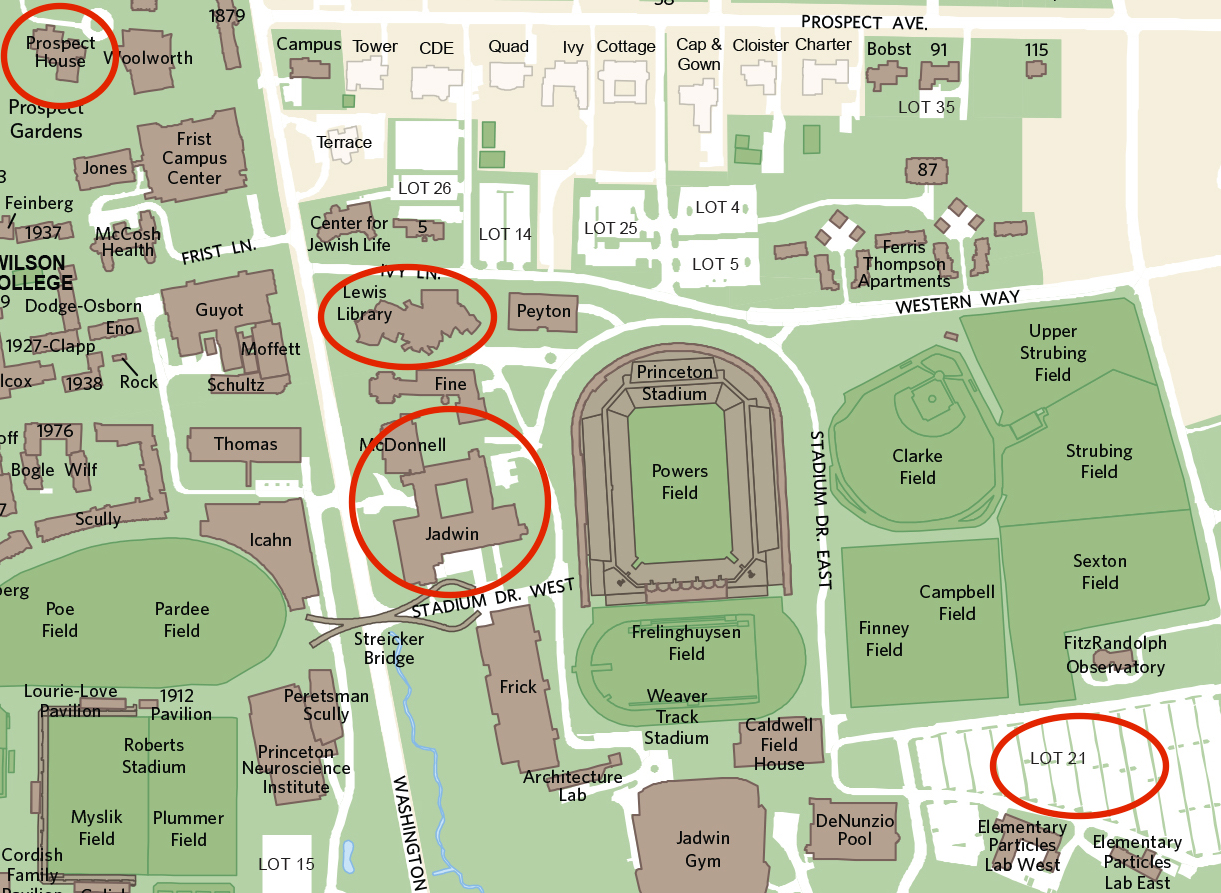
\includegraphics[width=0.8\textwidth]{images/PU-map-venues.jpeg}
%\caption{}
%\label{fig:example2}
\end{center}
\end{figure}

\end{frame}



%
%\begin{frame}
\frametitle{Google docs for live notes}

We have found it is useful to use a google doc to capture live notes during these workshops. 
\vskip 0.15in
See "Live Notes" on the workshop website (\url{https://indico.cern.ch/event/622920/}) for links to the google docs. You should join the S2I2-HEP google group in order to edit them.
\vskip 0.15in
There is one doc to use for the plenary session (Mon/Wed) and one google doc for each of the parallel sessions. Please feel free to contribute!

\end{frame}



%
%\begin{frame}
\frametitle{Participant Introduction Slides}

If you have not done so already, please fill out the short ``introduction''
slide about yourself. 
%\vskip 0.15in
\begin{figure}[htbp]
\begin{center}
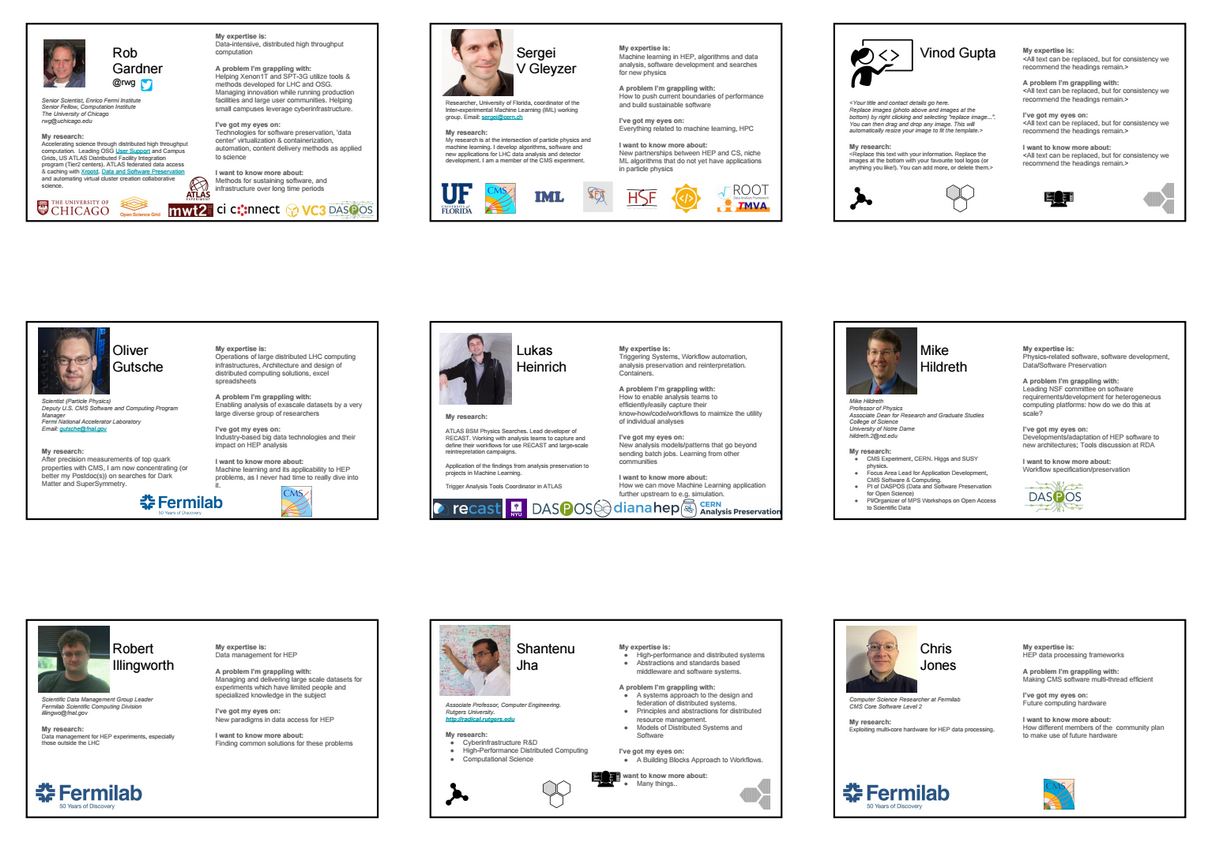
\includegraphics[width=0.6\textwidth]{images/s2i2-hep-cs-intros-page.png}
%\caption{}
%\label{fig:example2}
\end{center}
\end{figure}
%\vskip 0.15in
Short URL of participant slide deck: \url{http://bit.ly/2pm5MQx}

\end{frame}



%
%\begin{frame}
\frametitle{Workshop Participants - Research Community}

\begin{figure}[htbp]
\begin{center}
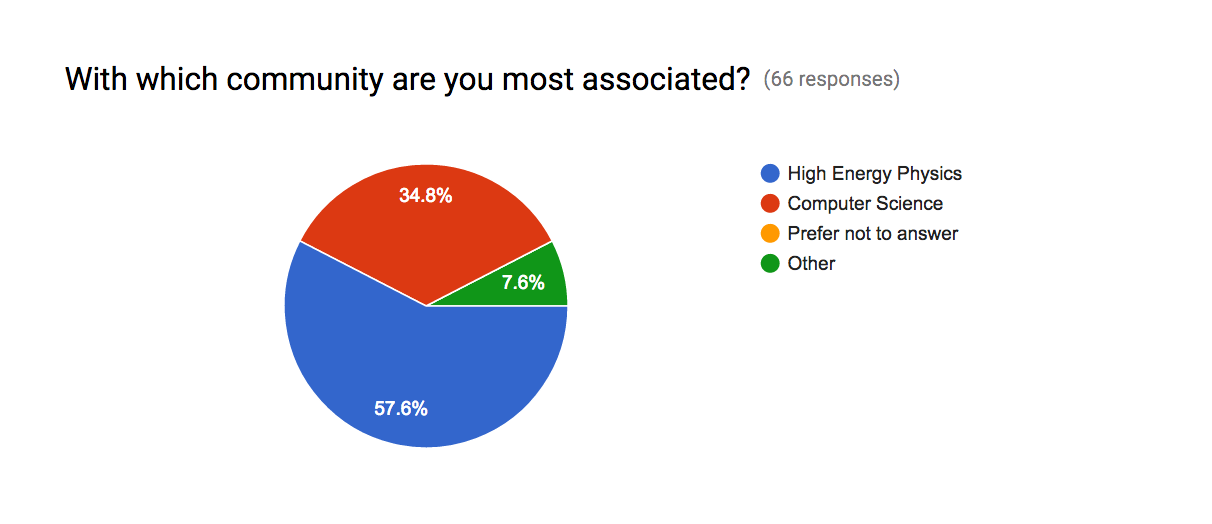
\includegraphics[width=1.0\textwidth]{images/s2i2-hep-cs-princeton-3-community.png}
%\caption{}
%\label{fig:example2}
\end{center}
\end{figure}

\end{frame}



%\begin{frame}
\frametitle{Workshop Participants - Institution Type}

\begin{figure}[htbp]
\begin{center}
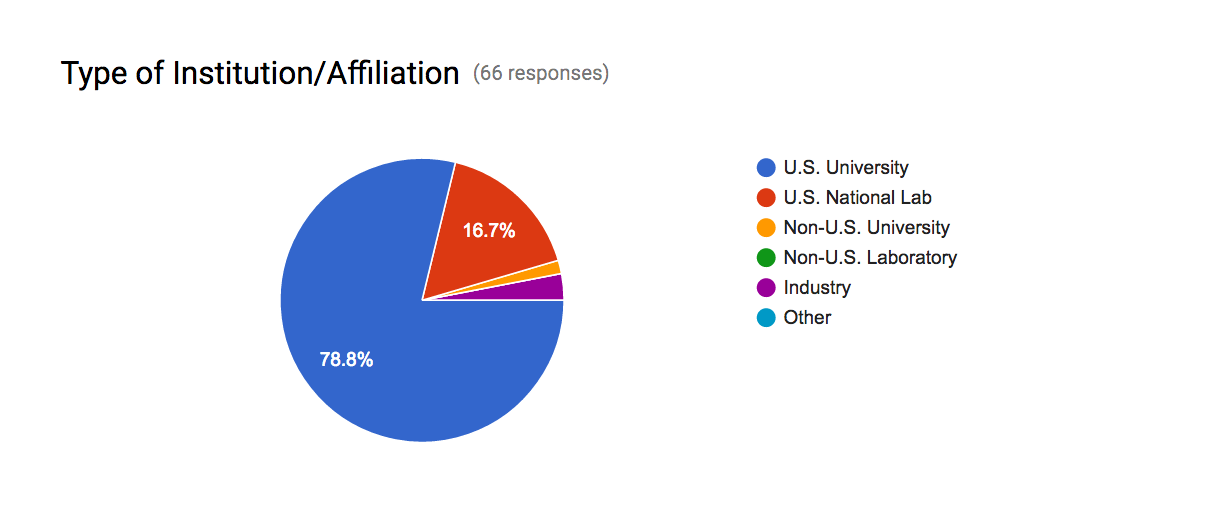
\includegraphics[width=1.0\textwidth]{images/s2i2-hep-cs-princeton-4-institution.png}
%\caption{}
%\label{fig:example2}
\end{center}
\end{figure}

\end{frame}



%\begin{frame}
\frametitle{Workshop Participants - Career Stage}

\begin{figure}[htbp]
\begin{center}
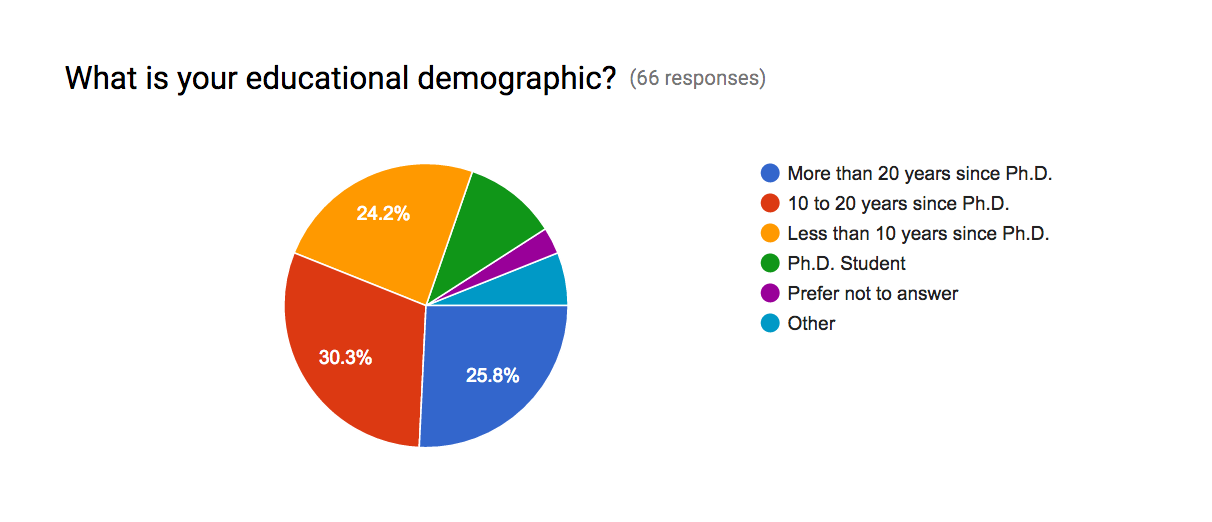
\includegraphics[width=1.0\textwidth]{images/s2i2-hep-cs-princeton-2-education.png}
%\caption{}
%\label{fig:example2}
\end{center}
\end{figure}

\end{frame}



%\begin{frame}
\frametitle{Workshop Participants - Session Interest}

\begin{figure}[htbp]
\begin{center}
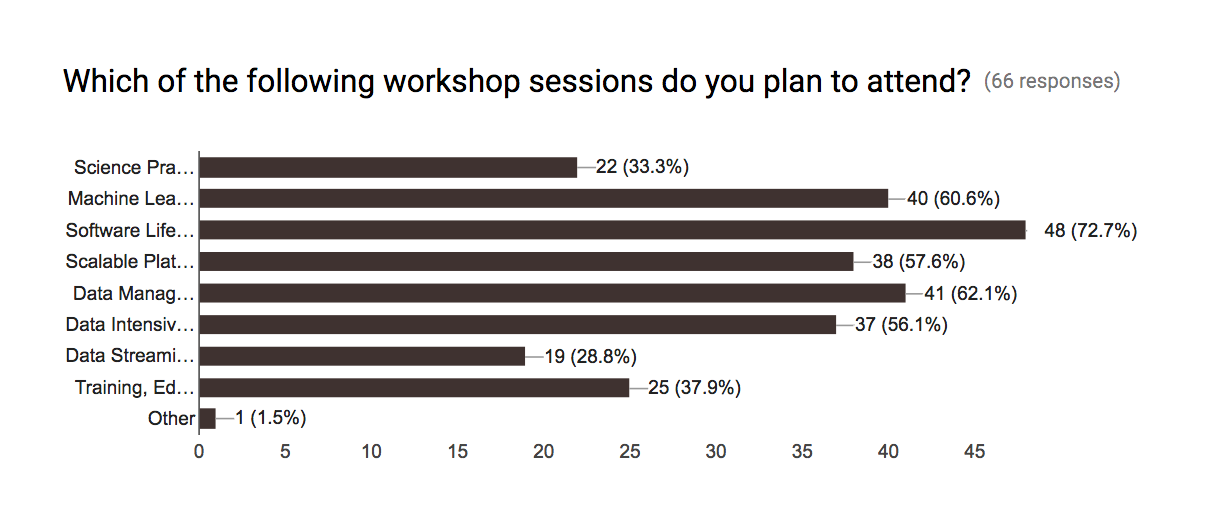
\includegraphics[width=1.0\textwidth]{images/s2i2-hep-cs-princeton-1-session-interest.png}
%\caption{}
%\label{fig:example2}
\end{center}
\end{figure}

\end{frame}




%\begin{frame}
\frametitle{NSF 15-553 - S2I2 Conceptualization Awards}

{\scriptsize
{\color{blue} (These) are planning
awards aimed at organizing an interdisciplinary community and
understanding their software requirements and challenges. (...)
The product of a conceptualization award will be a
strategic plan for enabling science and education through a sustained
software infrastructure that will be freely available to the
community, and will address the following elements:}

\begin{itemize}
\item the science community and the specific grand challenge research questions that the S2I2 will support;
\item specific software elements and frameworks that are relevant to the community, the sustainability challenges that need to be addressed, and why addressing these challenges will be transformative;
\item appropriate software architectures and lifecycle processes, development, testing and deployment methodologies, validation and verification processes, end usability and interface considerations, and required infrastructure and technologies;
\item the required organizational, personnel and management structures and operational processes;
\item the requirements and necessary mechanisms for human resource development, including integration of education and training, mentoring of students, postdoctoral fellows as well as software professionals, and proactively addressing diversity and broadening participation;
\item potential approaches for long-term sustainability of the software institute as well as the software; and
\item potential risks including risks associated with establishment and execution, necessary infrastructure and associated technologies, community engagement, and long-term sustainability.
\end{itemize}
}

\end{frame}



%\begin{frame}
\frametitle{NSF 15-553 - S2I2 Conceptualization Awards}

{\scriptsize
(These) are planning
awards aimed at organizing an interdisciplinary community and
understanding their software requirements and challenges. (...)
The product of a conceptualization award will be a
strategic plan for enabling science and education through a sustained
software infrastructure that will be freely available to the
community, and will address the following elements:

\begin{itemize}
\item {\color{blue} the science community and the specific grand challenge research questions that the S2I2 will support;}
\item specific software elements and frameworks that are relevant to the community, the sustainability challenges that need to be addressed, and why addressing these challenges will be transformative;
\item appropriate software architectures and lifecycle processes, development, testing and deployment methodologies, validation and verification processes, end usability and interface considerations, and required infrastructure and technologies;
\item the required organizational, personnel and management structures and operational processes;
\item the requirements and necessary mechanisms for human resource development, including integration of education and training, mentoring of students, postdoctoral fellows as well as software professionals, and proactively addressing diversity and broadening participation;
\item potential approaches for long-term sustainability of the software institute as well as the software; and
\item potential risks including risks associated with establishment and execution, necessary infrastructure and associated technologies, community engagement, and long-term sustainability.
\end{itemize}
}

\end{frame}



%\begin{frame}
\frametitle{NSF 15-553 - S2I2 Conceptualization Awards}

{\scriptsize
(These) are planning
awards aimed at organizing an interdisciplinary community and
understanding their software requirements and challenges. (...)
The product of a conceptualization award will be a
strategic plan for enabling science and education through a sustained
software infrastructure that will be freely available to the
community, and will address the following elements:

\begin{itemize}
\item the science community and the specific grand challenge research questions that the S2I2 will support;
\item {\color{blue} specific software elements and frameworks that are relevant to the community, the sustainability challenges that need to be addressed, and why addressing these challenges will be transformative;}
\item appropriate software architectures and lifecycle processes, development, testing and deployment methodologies, validation and verification processes, end usability and interface considerations, and required infrastructure and technologies;
\item the required organizational, personnel and management structures and operational processes;
\item the requirements and necessary mechanisms for human resource development, including integration of education and training, mentoring of students, postdoctoral fellows as well as software professionals, and proactively addressing diversity and broadening participation;
\item potential approaches for long-term sustainability of the software institute as well as the software; and
\item potential risks including risks associated with establishment and execution, necessary infrastructure and associated technologies, community engagement, and long-term sustainability.
\end{itemize}
}

\end{frame}



%\begin{frame}
\frametitle{NSF 15-553 - S2I2 Conceptualization Awards}

{\scriptsize
(These) are planning
awards aimed at organizing an interdisciplinary community and
understanding their software requirements and challenges. (...)
The product of a conceptualization award will be a
strategic plan for enabling science and education through a sustained
software infrastructure that will be freely available to the
community, and will address the following elements:

\begin{itemize}
\item the science community and the specific grand challenge research questions that the S2I2 will support;
\item specific software elements and frameworks that are relevant to the community, the sustainability challenges that need to be addressed, and why addressing these challenges will be transformative;
\item appropriate software architectures and lifecycle processes, development, testing and deployment methodologies, validation and verification processes, end usability and interface considerations, and required infrastructure and technologies;
\item {\color{blue} the required organizational, personnel and management structures and operational processes;}
\item the requirements and necessary mechanisms for human resource development, including integration of education and training, mentoring of students, postdoctoral fellows as well as software professionals, and proactively addressing diversity and broadening participation;
\item potential approaches for long-term sustainability of the software institute as well as the software; and
\item potential risks including risks associated with establishment and execution, necessary infrastructure and associated technologies, community engagement, and long-term sustainability.
\end{itemize}
}

\end{frame}



%\begin{frame}
\frametitle{NSF 15-553 - S2I2 Conceptualization Awards}

{\scriptsize
(These) are planning
awards aimed at organizing an interdisciplinary community and
understanding their software requirements and challenges. (...)
The product of a conceptualization award will be a
strategic plan for enabling science and education through a sustained
software infrastructure that will be freely available to the
community, and will address the following elements:

\begin{itemize}
\item the science community and the specific grand challenge research questions that the S2I2 will support;
\item specific software elements and frameworks that are relevant to the community, the sustainability challenges that need to be addressed, and why addressing these challenges will be transformative;
\item {\color{blue} appropriate software architectures and lifecycle processes, development, testing and deployment methodologies, validation and verification processes, end usability and interface considerations, and required infrastructure and technologies;}
\item the required organizational, personnel and management structures and operational processes;
\item {\color{blue} the requirements and necessary mechanisms for human resource development, including integration of education and training, mentoring of students, postdoctoral fellows as well as software professionals, and proactively addressing diversity and broadening participation;}
\item {\color{blue} potential approaches for long-term sustainability of the software institute as well as the software; and}
\item {\color{blue} potential risks including risks associated with establishment and execution, necessary infrastructure and associated technologies, community engagement, and long-term sustainability.}
\end{itemize}
}

\end{frame}




% S2I2 HEP introdution

\begin{frame}
\frametitle{S2I2-HEP}
The primary goal of the S2I2-HEP conceptualization project (\url{http://s2i2-hep.org}) is to produce a well-defined strategy for R\&D for the software and computing models for use in high energy physics (HEP), in particular for the experiments collecting the very large data sets anticipated in the ``High-Luminosity Large Hadron Collider'' (HL-LHC) era of the 2020s. \\
\vskip 0.15in
Specifically the S2I2-HEP project will identify potential areas where U.S. university personnel can lead in key areas of software development to help realize the full potential of the HL-LHC program. \\
\vskip 0.15in
However HEP and the LHC are global projects, so no long-term planning exercise can exist in isolation, thus we are also pursuing a wider HEP community roadmap for software and computing in the 2020s.
\end{frame}



\begin{frame}
\frametitle{LHC Grand Challenge Research Questions}

The goal of HEP (and the LHC) is to understand the fundamental building blocks of nature, and their interactions. The potential of the LHC has been demonstrated in its first years with the discovery of the Higgs Boson. \\
\vskip 0.15in
\begin{figure}[htbp]
\begin{center}
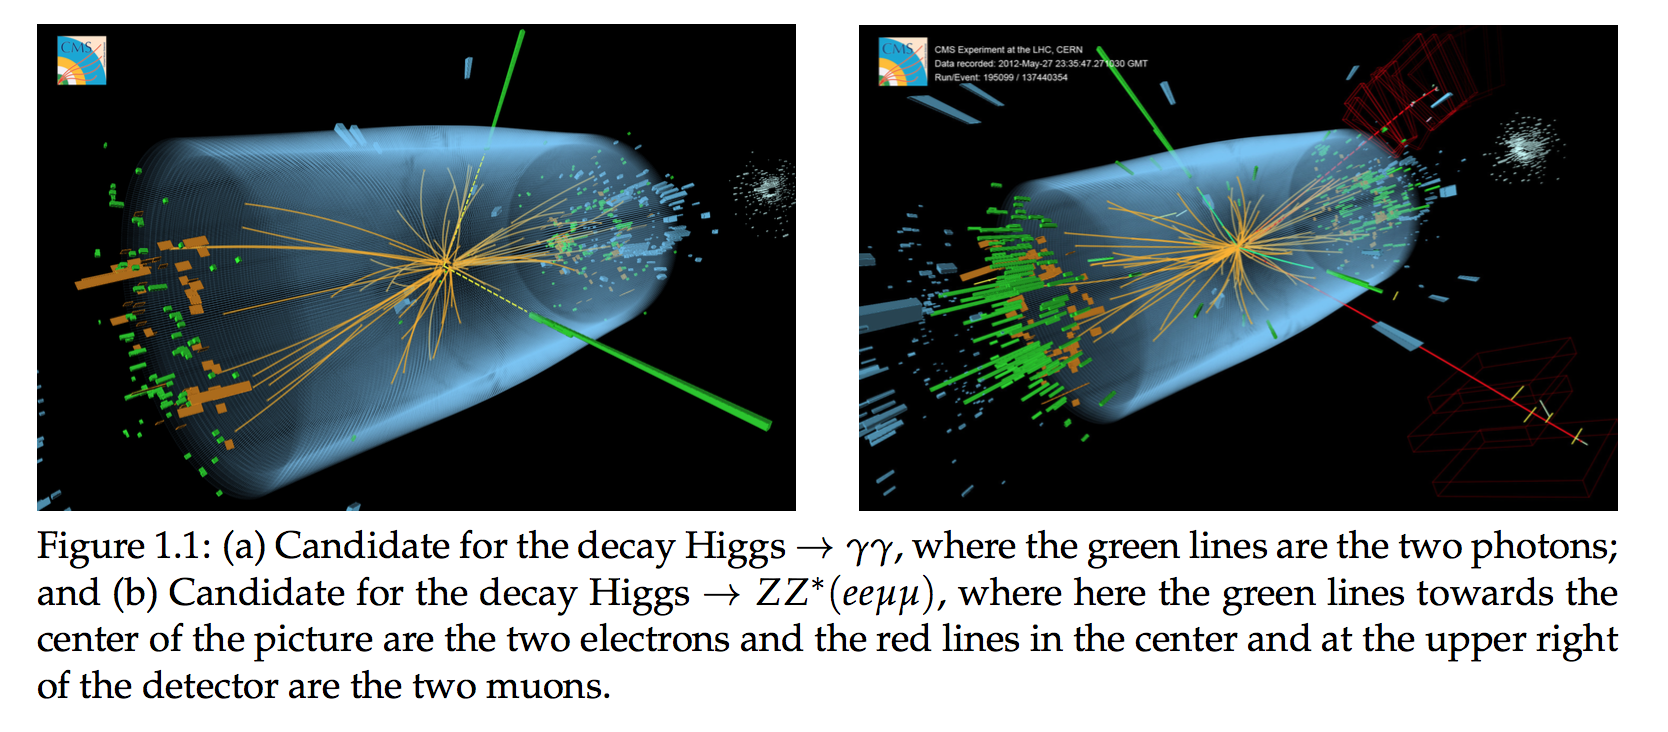
\includegraphics[width=1.0\textwidth]{images/cms-higgs-events.png}
%\caption{}
%\label{fig:example2}
\end{center}
\end{figure}

\end{frame}



\begin{frame}
\frametitle{LHC Grand Challenge Research Questions}

Many fundamental questions remain, however, including: Why does nature express the symmetries embodied in the SM, and not other equally elegant symmetries? Why are there (only) three generations of basic building blocks of matter? Why are the masses of these building blocks so different from each other, both within a generation and between generations? What is the dark matter which pervades the Universe? Why is matter so dominant over antimatter in the Universe? Does space-time have additional symmetries or extend beyond the 3+1 dimensions of which we know? What mechanism stabilizes the Higgs mass from large quantum corrections at high energy? Are neutrinos their own anti-particles? Can gravity and quantum mechanics be described in a consistent theoretical framework?

\end{frame}



\begin{frame}
\frametitle{Large Hadron Collider (LHC) and Experiments}

\begin{figure}[htbp]
\begin{center}
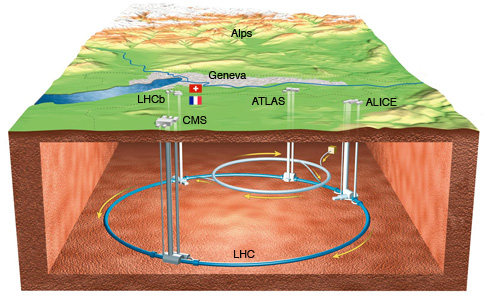
\includegraphics[width=0.8\textwidth]{images/CERNMap.jpg}
%\caption{}
%\label{fig:example2}
\end{center}
\end{figure}

\small{Two very large experiments (Atlas, CMS) with 3500+ people, and two large experiments (Alice, LHCb) with 500+ people}

\end{frame}



\begin{frame}
\frametitle{WLCG Distributed Computing System}

\begin{figure}[htbp]
\begin{center}
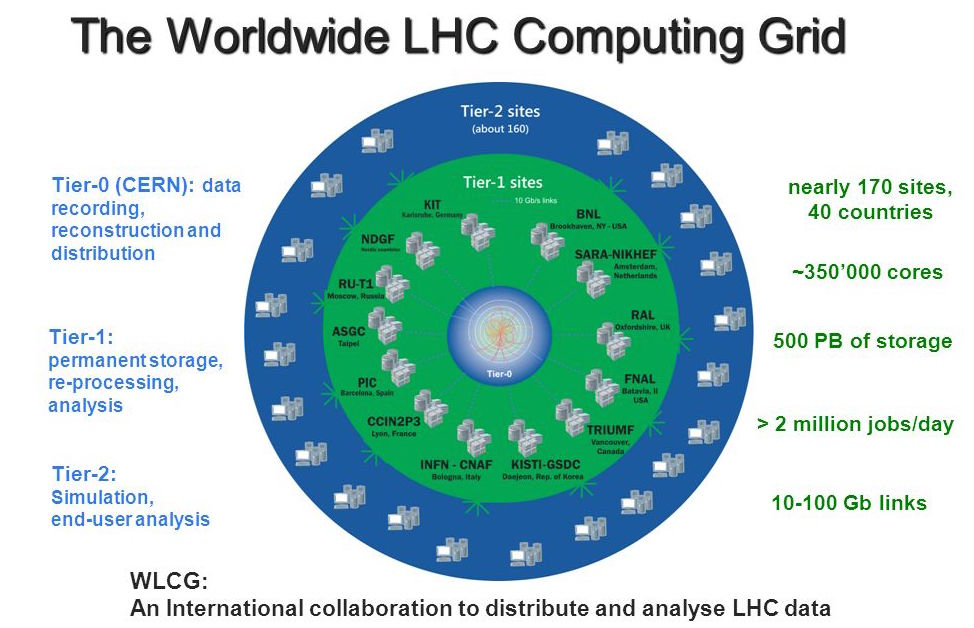
\includegraphics[width=0.9\textwidth]{images/wlcg-2015.jpeg}
%\caption{}
%\label{fig:example2}
\end{center}
\end{figure}

\small{Slide from 2015}

\end{frame}



%\begin{frame}
\frametitle{CERN Accelerator Timeline}

\begin{figure}[htbp]
\begin{center}
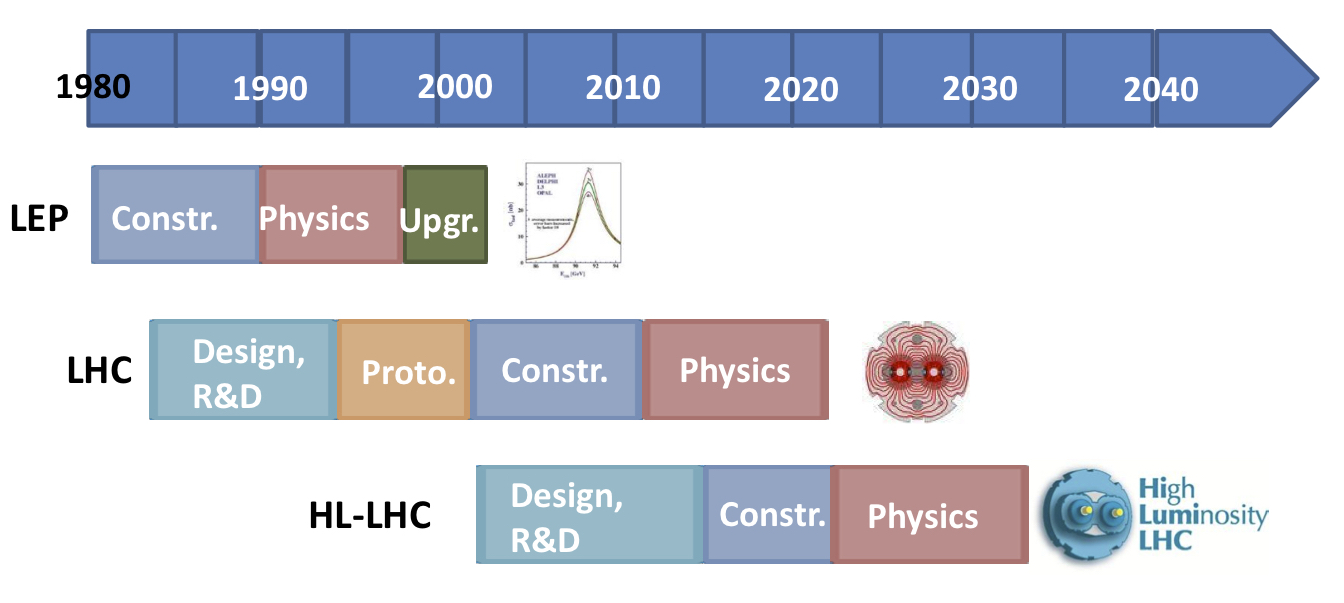
\includegraphics[width=1.0\textwidth]{images/timelineCERNprojects_image_current.jpg}
%\caption{}
%\label{fig:example2}
\end{center}
\end{figure}

\small{Various concepts also exist for subsequent machines.}

\end{frame}



\begin{frame}
\frametitle{Plans for upgrading the LHC and Experiment Detectors}

\begin{figure}[htbp]
\begin{center}
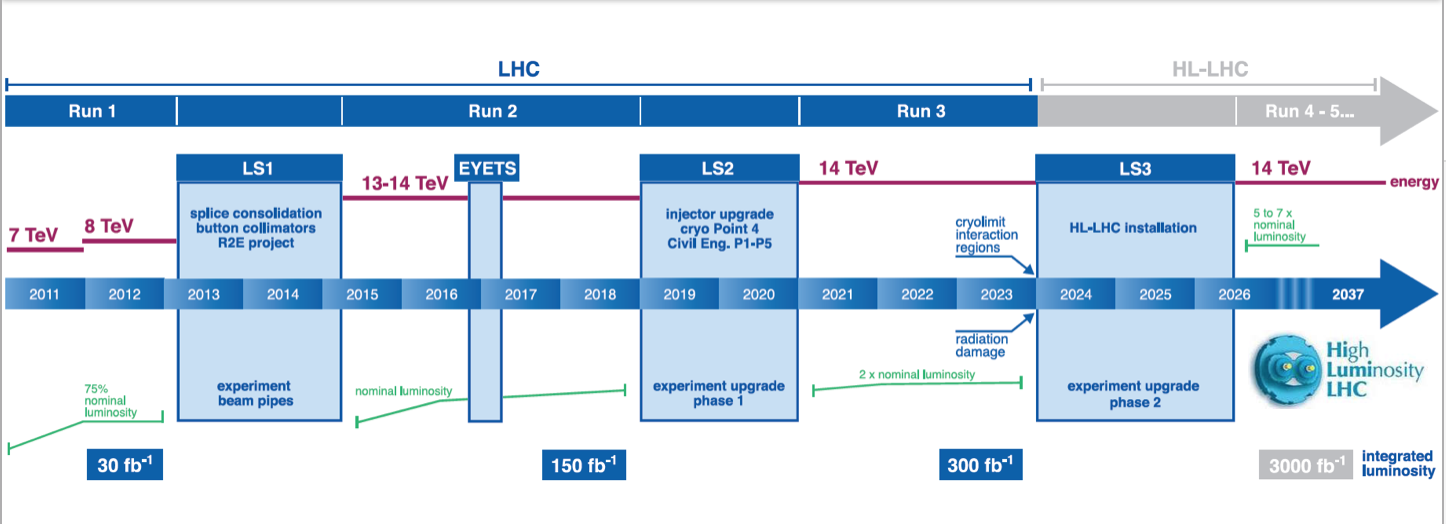
\includegraphics[width=1.0\textwidth]{images/lhc-upgrade-timeline-detail.png}
%\caption{}
%\label{fig:example2}
\end{center}
\end{figure}

%\small{Example Text}

\end{frame}



%\begin{frame}
\frametitle{Plans for upgrading the LHC and Experiment Detectors}

\begin{figure}[htbp]
\begin{center}
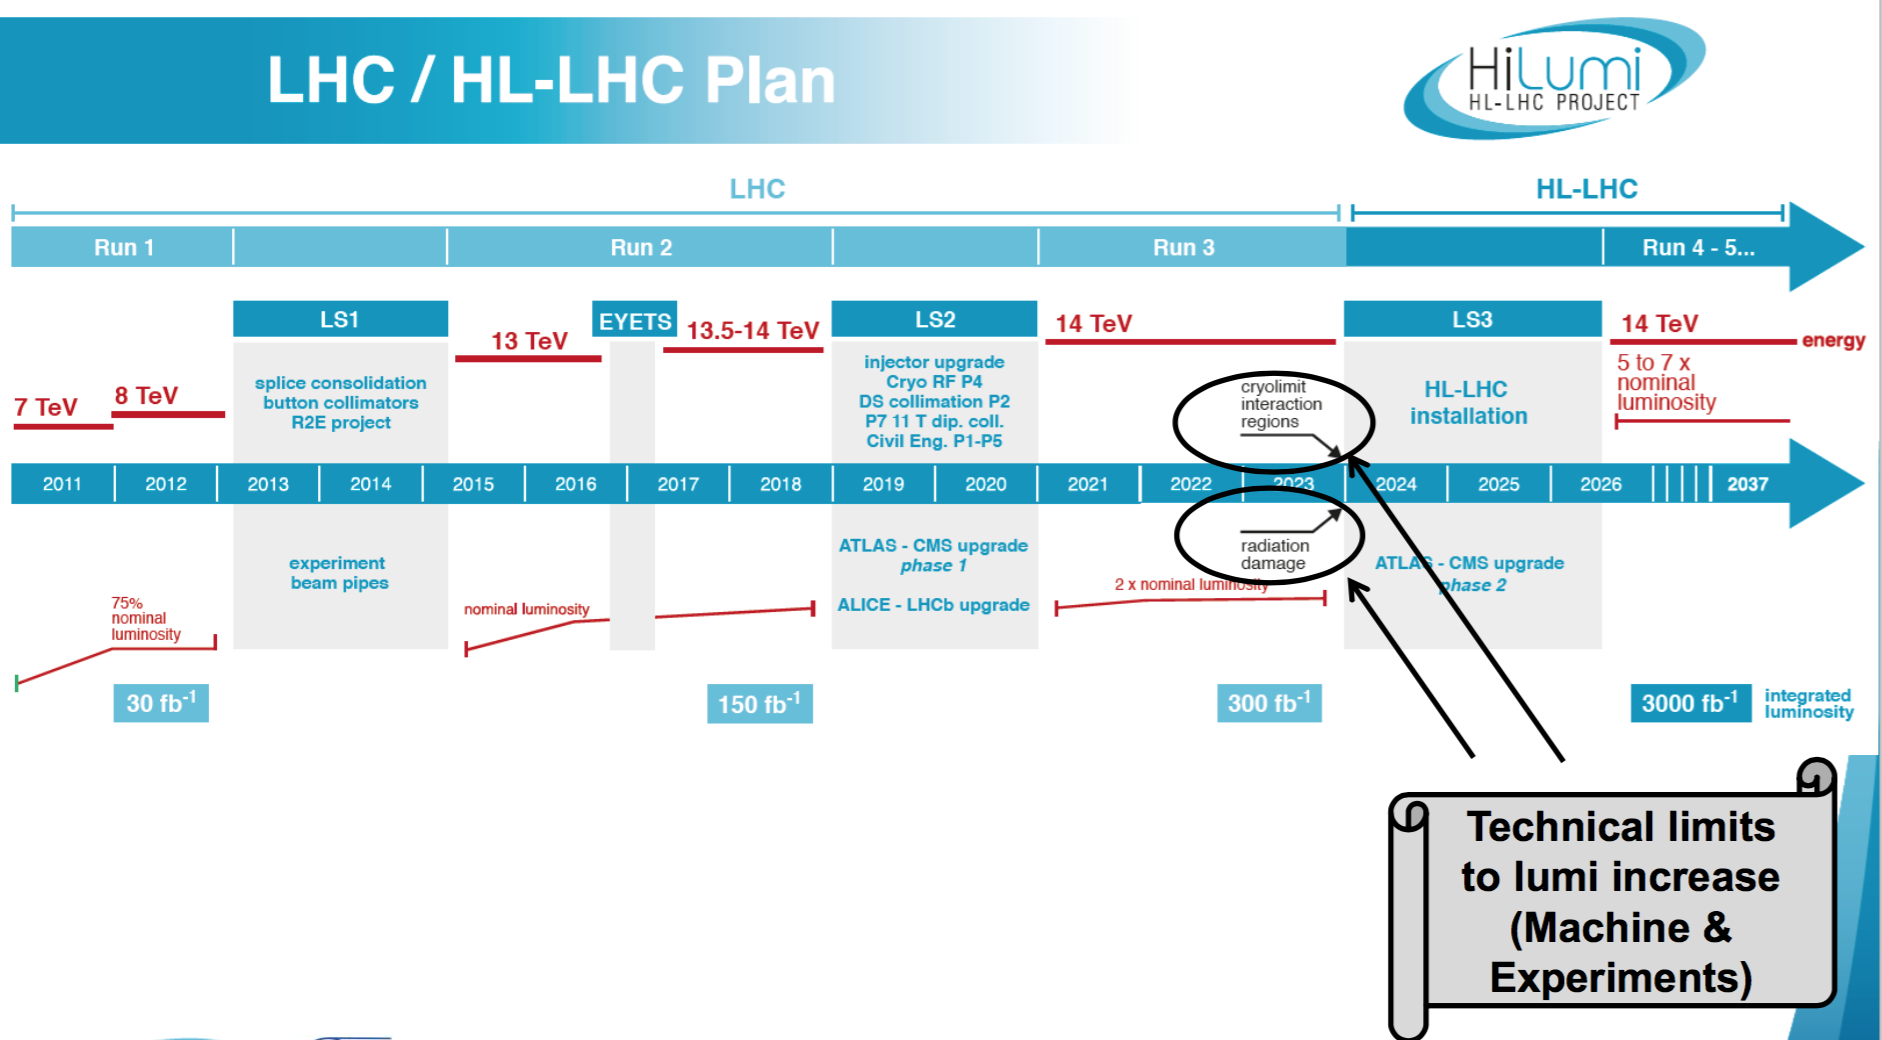
\includegraphics[width=0.9\textwidth]{images/20170202-rossi-hllhc-2.png}
%\caption{}
%\label{fig:example2}
\end{center}
\end{figure}

%\small{Example Text}

\end{frame}



\begin{frame}
\frametitle{Plans for upgrading the LHC and Experiment Detectors}

\begin{figure}[htbp]
\begin{center}
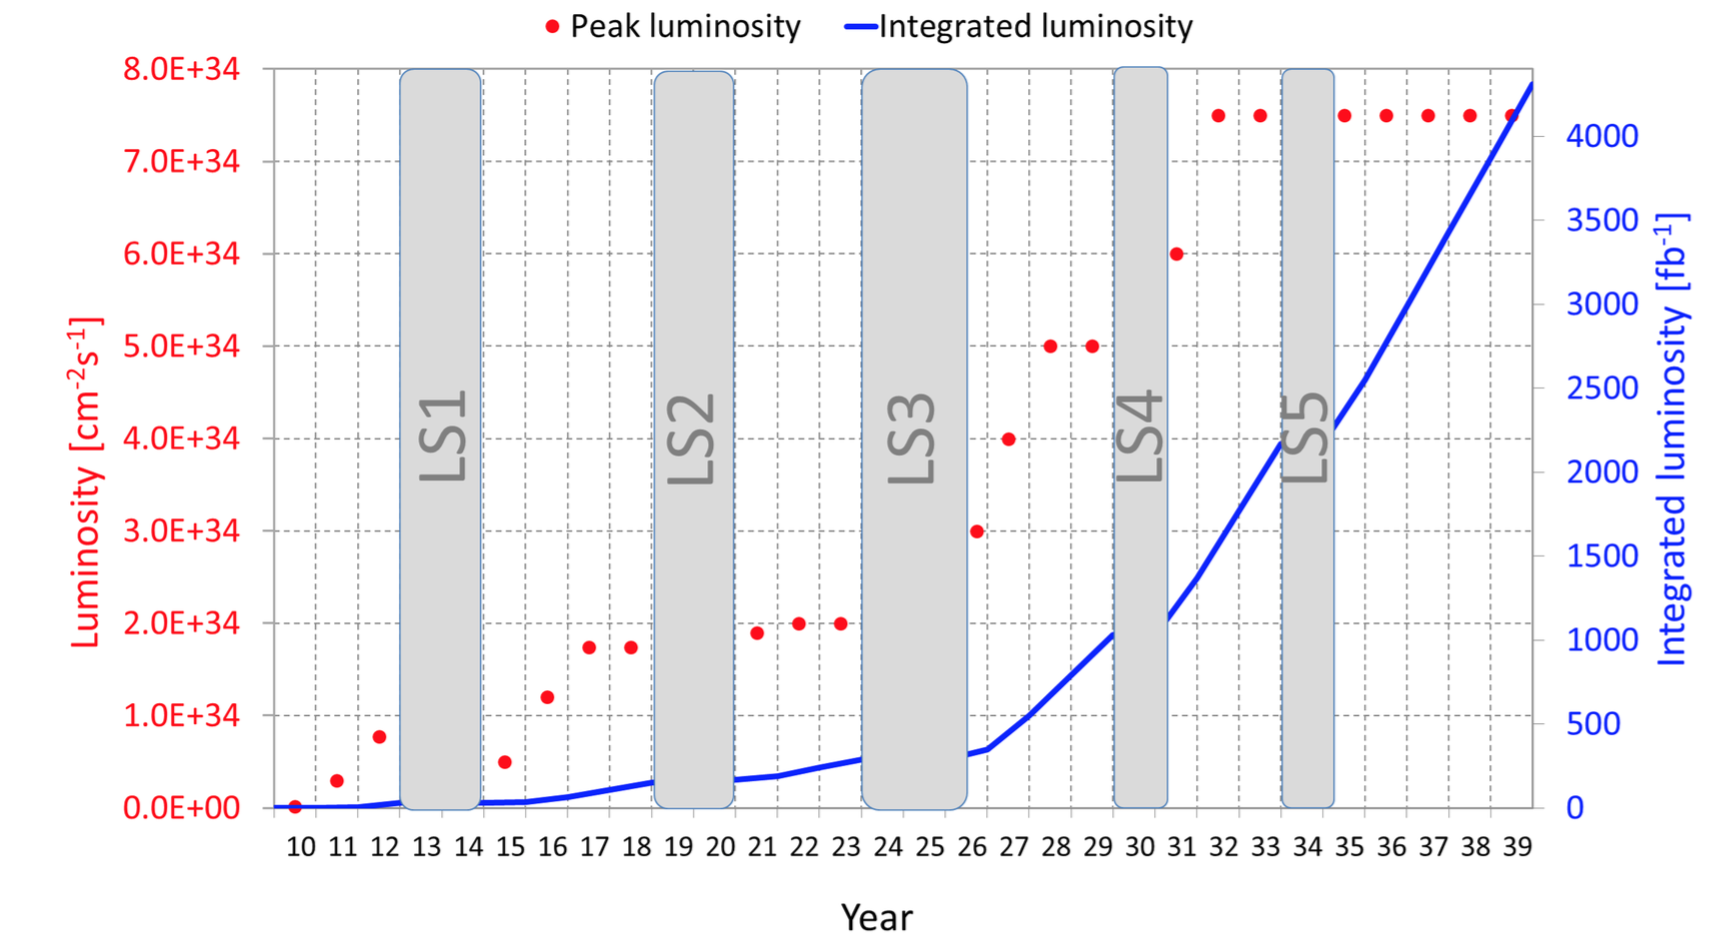
\includegraphics[width=0.9\textwidth]{images/20170202-rossi-hllhc-1.png}
%\caption{}
%\label{fig:example2}
\end{center}
\end{figure}

%\small{Example Text}

\end{frame}



\begin{frame}
\frametitle{A Software ``Upgrade'' for HL-LHC and 2020s HEP?}

Looking forward to the next 10 years, we see a number of challenges for HEP software and computing:

\begin{itemize}
\item {\bf Performance/cost:} Estimates of computing needs run faster than Moore's Law by factors of o(10)
\item {\bf Technology/Market evolution:} the return of heterogeneity; technology change will also make it challenging to exploit Moore's Law without software evolution.
\item {\bf Scale:} The HL-LHC will integrate 100 times the current data, with significantly increased data (pileup) and detector complexity.
\item {\bf Sustainability:} Most of the current software, which defines our capabilities, was designed 15-20 years ago: there are many software sustainability challenges.
\end{itemize}

\end{frame}



\begin{frame}
\frametitle{Estimates of Resource Needs for HL-LHC (WLCG)}

\begin{figure}[htbp]
\begin{center}
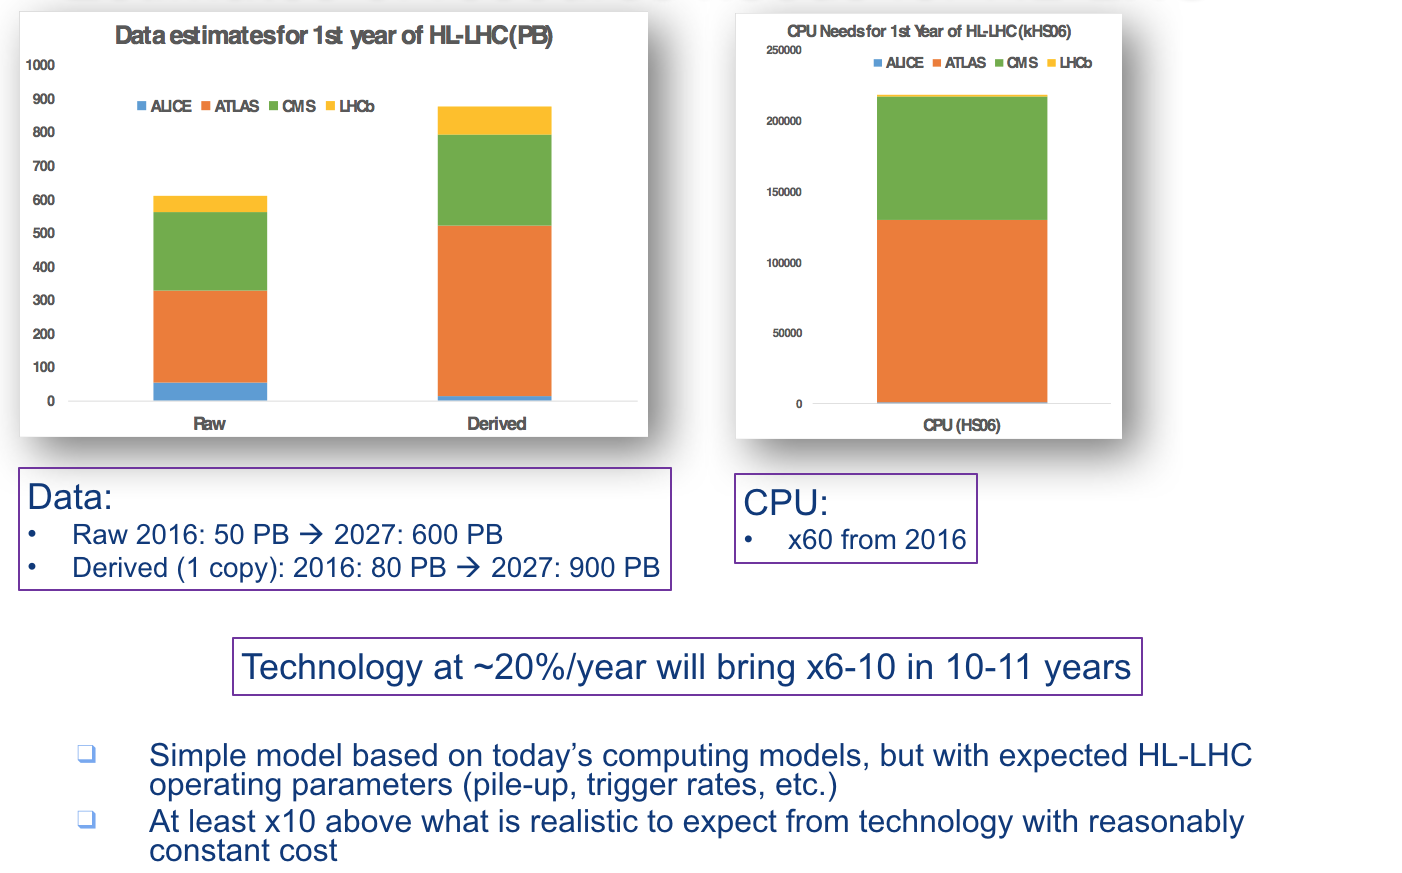
\includegraphics[width=0.9\textwidth]{images/20161008-wlcg-intro-ian-bird-slide-10.png}
\end{center}
\end{figure}

\begin{center}
\small{(Slide from WLCG Workshop Intro, Ian Bird, 8 Oct, 2016)}
\end{center}

\end{frame}




\begin{frame}
\frametitle{CPU and bulk processing capacity}

The vast majority of the CPU needs at the HL-LHC come from pattern recognition algorithms (``reconstruction'' for HEP). This probably a factor of 10 short, assuming we get and can exploit 20\%/year Moore's Law gains.

\begin{figure}[htbp]
\begin{center}
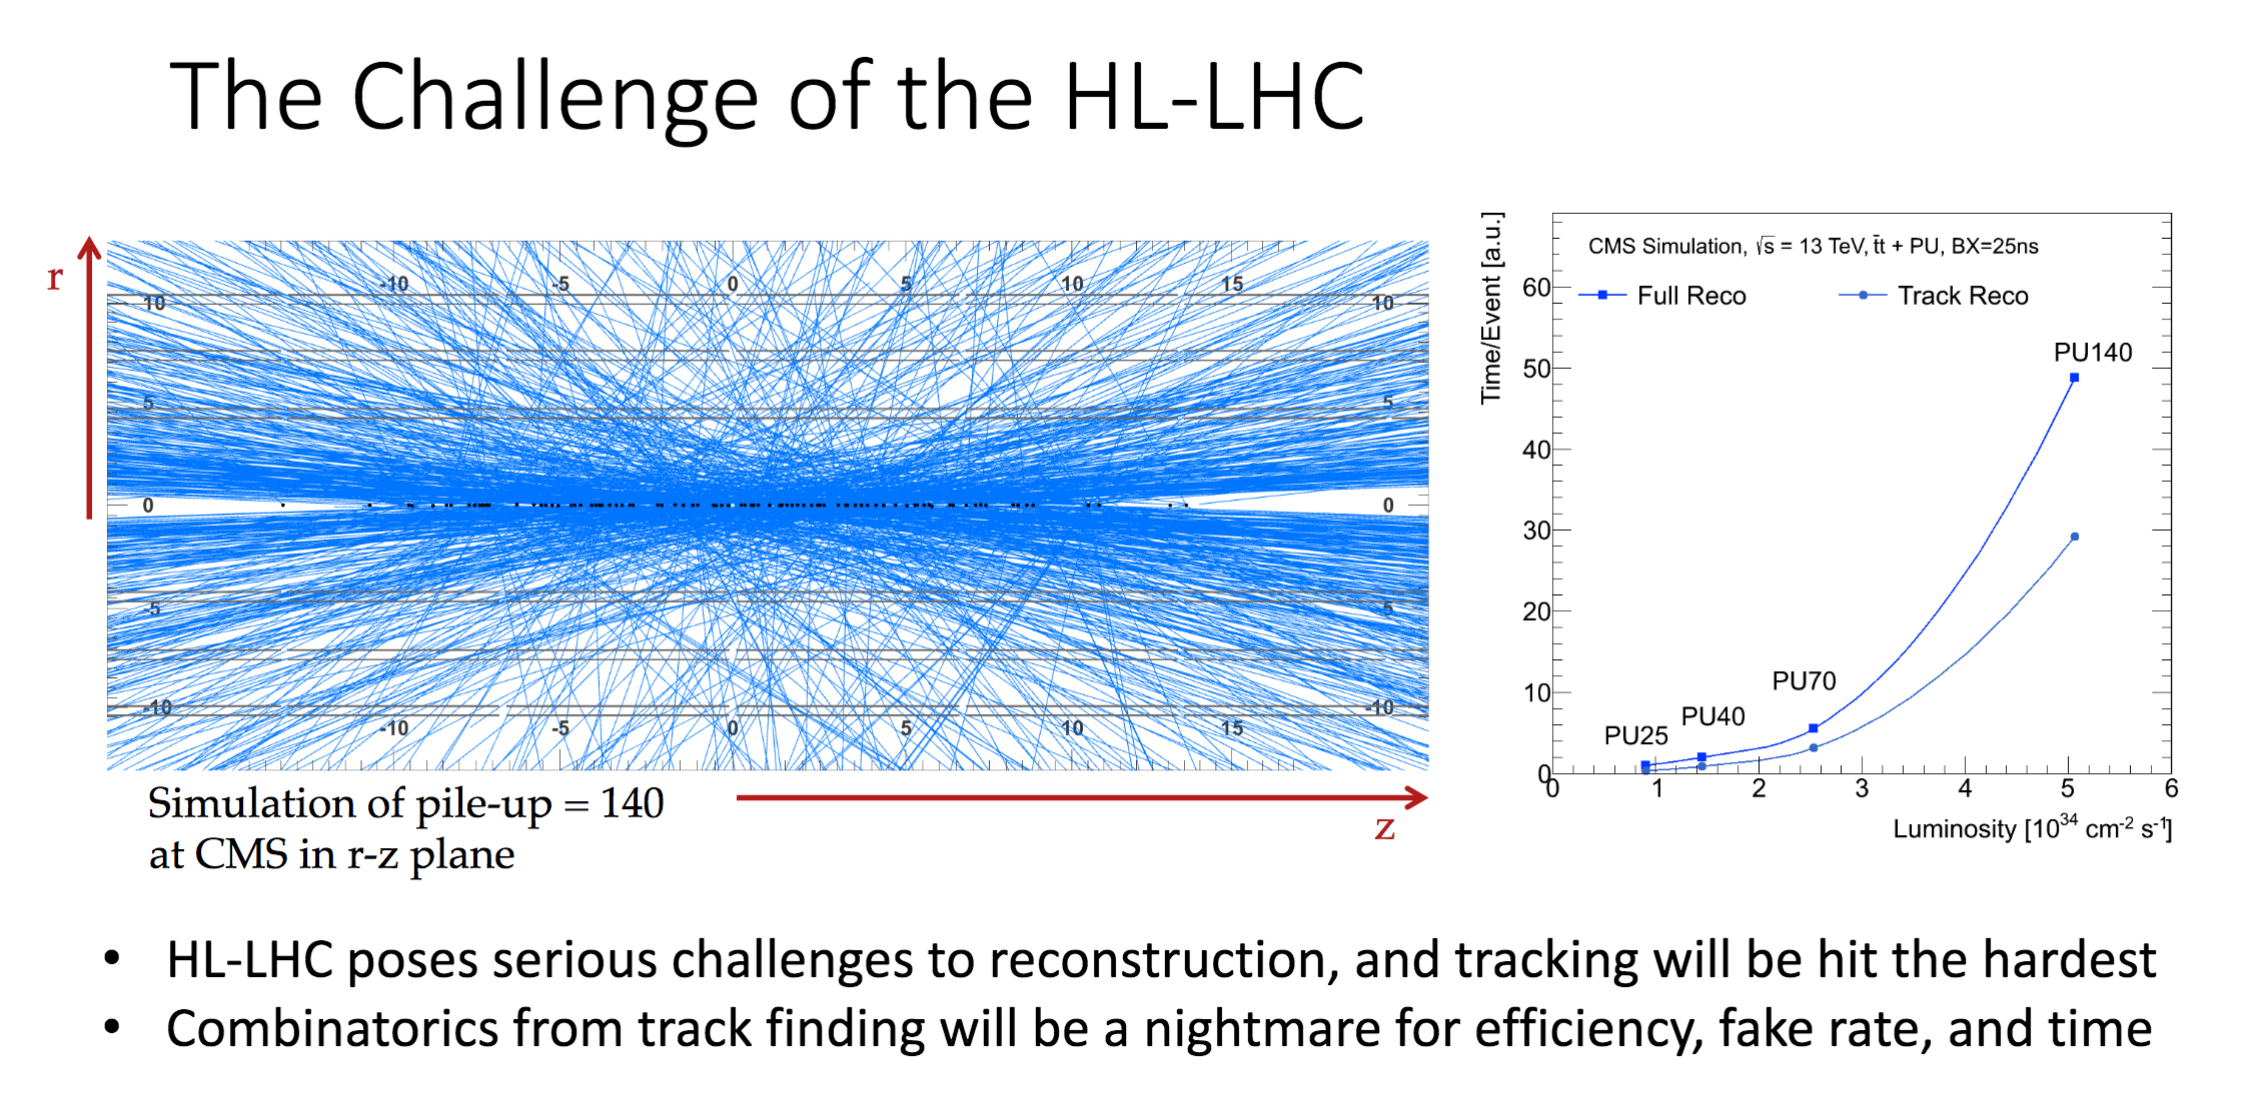
\includegraphics[width=1.0\textwidth]{images/hllhc-reco-tracking.png}
%\caption{}
%\label{fig:example2}
\end{center}
\end{figure}

\end{frame}




\begin{frame}
\frametitle{Processor evolution and software impact}

\begin{columns}[T] % align columns

\begin{column}{.48\textwidth}
\begin{figure}[htbp]
\begin{center}
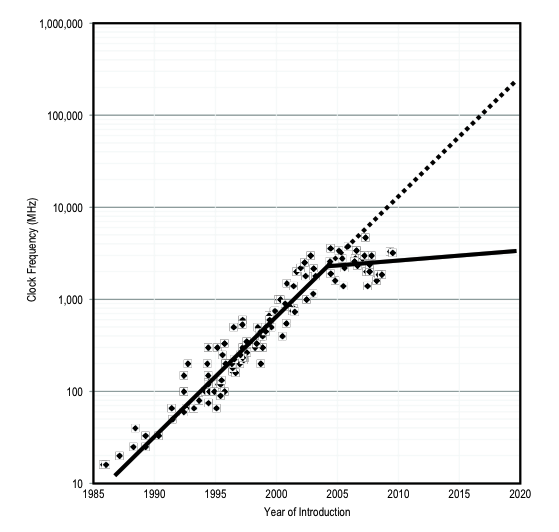
\includegraphics[width=1.0\textwidth]{images/moore2.png}
\end{center}
\end{figure}
\begin{center}
\small{Clock Frequency vs Time}
\end{center}
\end{column}%

\hfill%

\begin{column}{.48\textwidth}
\begin{itemize}
\item Single core performance has stalled, leading to multi/manycore and specialization
\item To even realize Moore's Law gains, we are pushed towards parallelization of algorithms and design for performance.
\item The software designs and implementations themselves need to evolve, not just be recompiled
\end{itemize}
\end{column}%

\end{columns}

\end{frame}



\begin{frame}
\frametitle{Back to heterogeneous systems?}

Building the worldwide distributed LHC computing grid was largely made possible by the convergence on Linux on (commodity) Intel x86 processors around the year 2000. Building the WLCG at this scale in the heterogeneous workstation era would have been quite difficult. For better or for worse, heterogeneity is returning:

\begin{itemize}
\item Diversity of computing processor architectures (general purpose cores vs specialized processors)
\item Owned vs commercial/cloud providers
\item Some pressure to use systems traditionally designed for other types of applications (e.g.\ HPC/supercomputer as opposed to HTC/high-throughput systems)
\item Possible further commoditizing market pressures (e.g. mobile)
\end{itemize}

\end{frame}




\begin{frame}
\frametitle{Data Access, Organization and Management}
Similarly managing and accessing a factor of 10 increase in data volume/year is a challenge. 
\vskip 0.15in
This can also be exacerbated by any evolution required to use processing capacity (Grid, Cloud, HPC center). The evolution of tape, networks and heterogeneous computing will likely a more dynamic model. Optimizations and trade-offs within that will be critical.

\end{frame}




\begin{frame}
\frametitle{Analysis Data Reduction - ``Last Mile''}

\begin{figure}[htbp]
\begin{center}
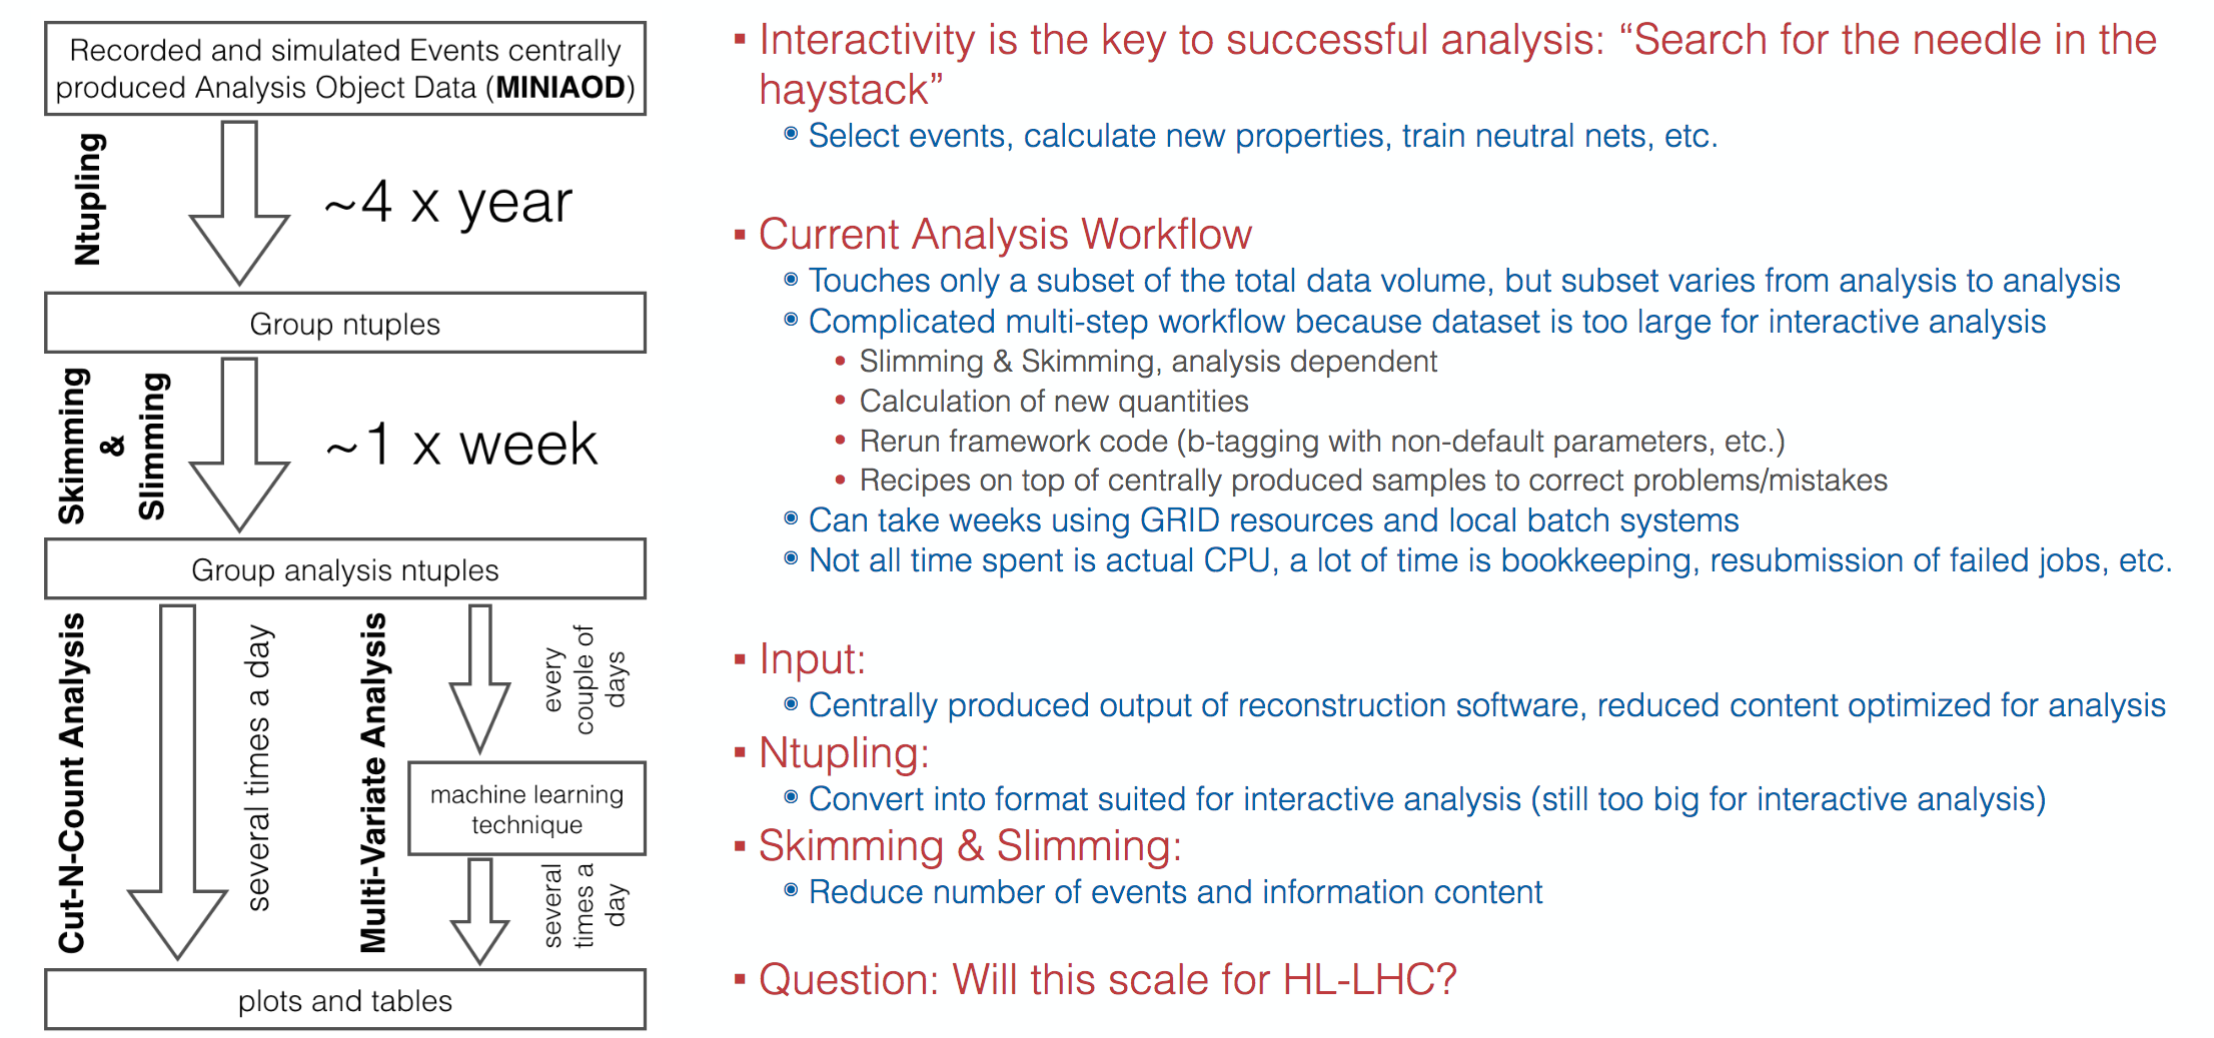
\includegraphics[width=1.0\textwidth]{images/analysis-data-reduction.png}
%\caption{}
%\label{fig:example2}
\end{center}
\end{figure}

\end{frame}




%\begin{frame}
\frametitle{What is software sustainability?} 
\begin{itemize}
\item {\bf Dependent Infrastructure:} Will the infrastructure element continue to provide the same functionality in the future, even when the other parts of the infrastructure on which the element relies change?
\item {\bf Collaborative Infrastructure} Can the element be combined with other elements to meet user needs, as both the collaborative elements and the individual elements change?
\item {\bf New Users:} Is the functionality and usability of the infrastructure element clearly explained to new users? Do users have a mechanism to ask questions and to learn about the element?
\item {\bf Existing Users:} Does the infrastructure element provide the functionality that current users want? Is it modular and adaptable so that it can meet the future needs of the users?
\item {\bf Science:} Does it incorporate and implement new science and theory as they develop?
\end{itemize}

\tiny{ Katz, D.S. \& Proctor, D., (2014). A Framework for Discussing e-Research Infrastructure Sustainability. Journal of Open Research Software. 2(1), p.e13. DOI: http://doi.org/10.5334/jors.av}
\end{frame}



\begin{frame}
\frametitle{Why Software? Software is {\em the} Cyberinfrastructure}

\begin{figure}[htbp]
\begin{center}
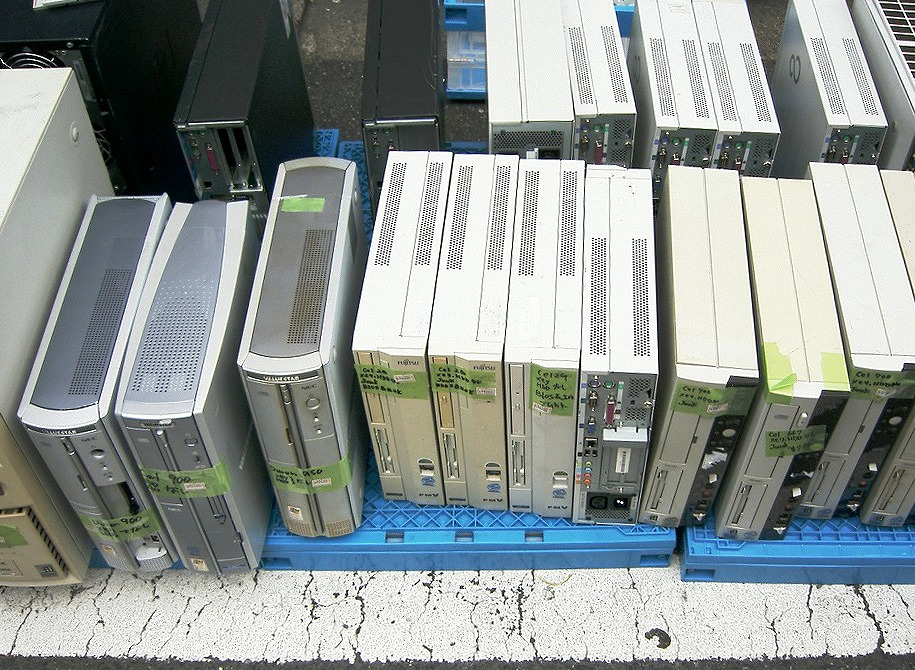
\includegraphics[width=0.7\textwidth]{images/Junk_desktop_personal_computer.jpg}
%\caption{}
%\label{fig:example2}
\end{center}
\end{figure}

\begin{center}
\small{Computer hardware is a consumable. \\ Software is what we keep, and invest in, over time.}
\end{center}

\end{frame}



\begin{frame}
\frametitle{HEP Software Ecosystem}

\begin{figure}[htbp]
\begin{center}
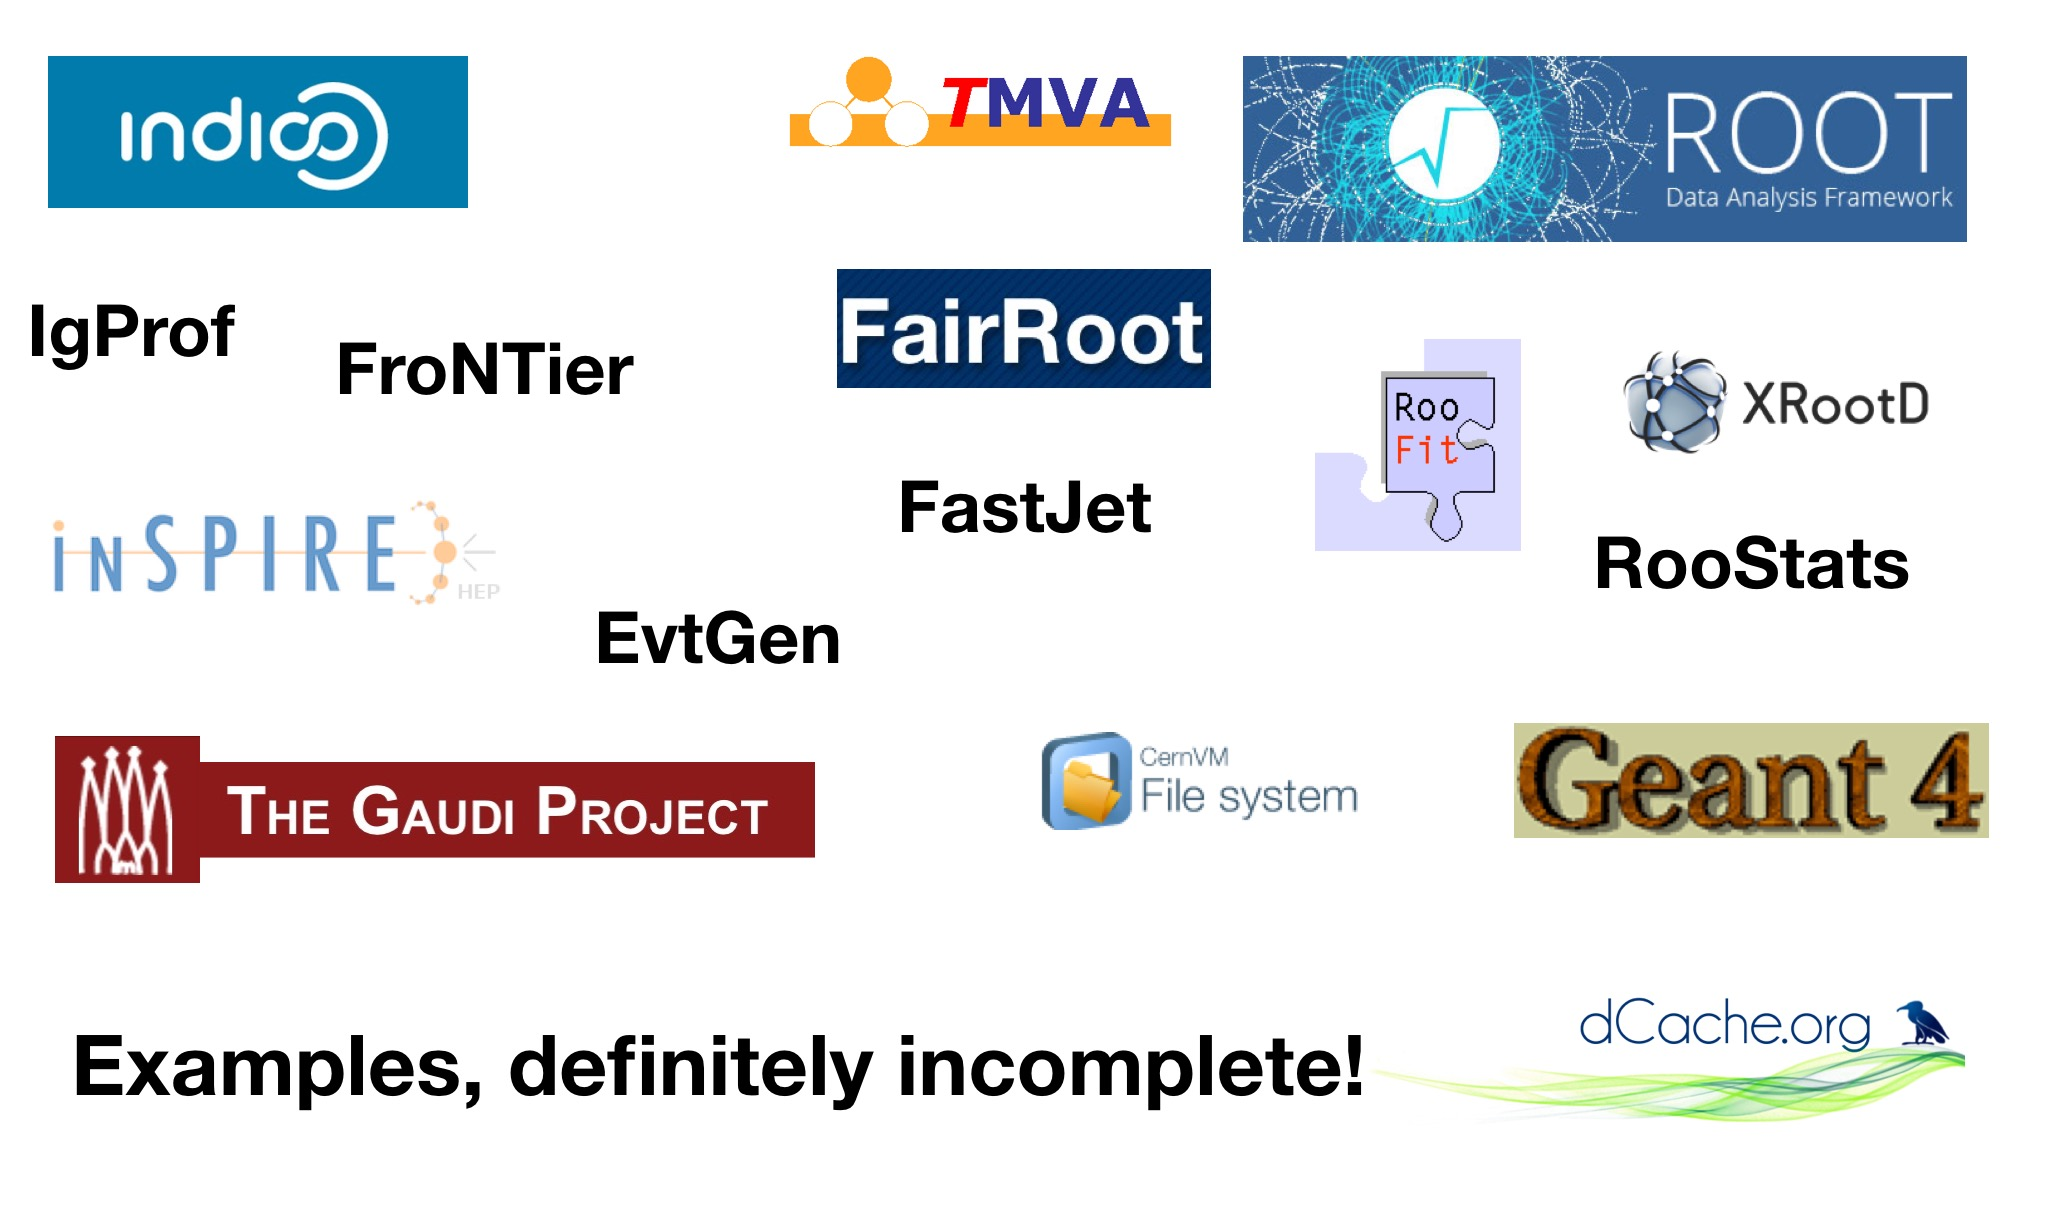
\includegraphics[width=0.9\textwidth]{images/hep-software-ecosystem.jpg}
\end{center}
\end{figure}

{\small Plus 15-20M Source Lines of Code (SLOC) of ``experiment specific'' codes, as well as dependencies on non-HEP scientific software.}
\end{frame}




%\begin{frame}
\frametitle{HEP Organization}

\begin{itemize}
\item HEP is organized at a global scale (``Big Science'') through experiments involving 100s to 1000s of invididuals. 
\item This can be daunting: how does one university group or grad student make an impact?
\item Building these large experiments has pushed HEP to create organizational structures that permit individuals to contribute.
\item The grad student will quickly and routinely wind up presenting to large groups of collaborators. Similarly, HEP has a footprint in 100+ computing centers around the world.
\item Other advantages: realistic computing/software problems at a large scale, relatively open academic culture.
\end{itemize}

\end{frame}



%\begin{frame}
\frametitle{HEP Organization}

\begin{figure}[htbp]
\begin{center}
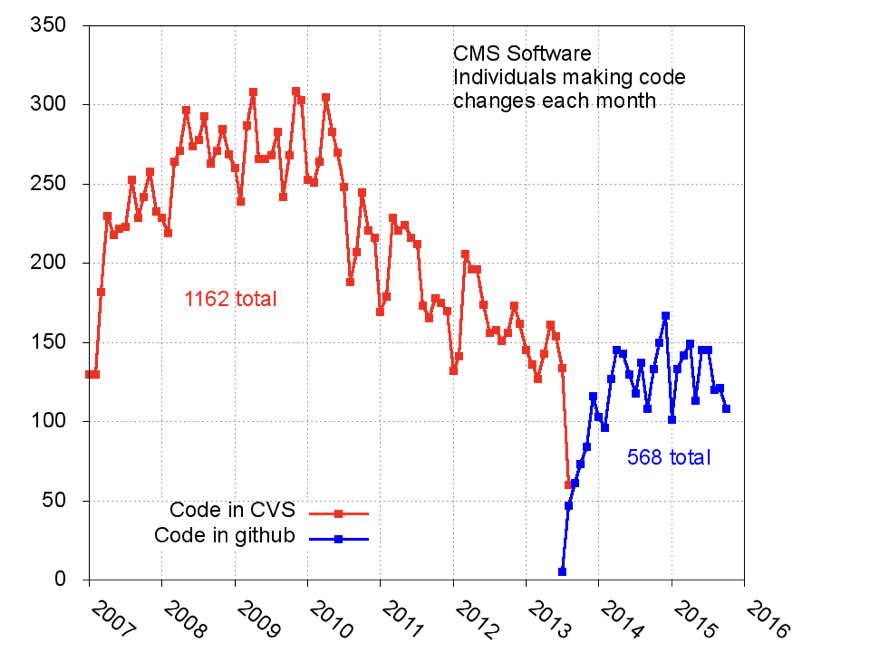
\includegraphics[width=0.8\textwidth]{images/cmssw-software-contributors-cvs-github.png}
%\caption{}
%\label{fig:example2}
\end{center}
\end{figure}

%\small{Example Text}

\end{frame}



%\begin{frame}
\frametitle{CERN Experiments in the 1990s}

\begin{figure}[htbp]
\begin{center}
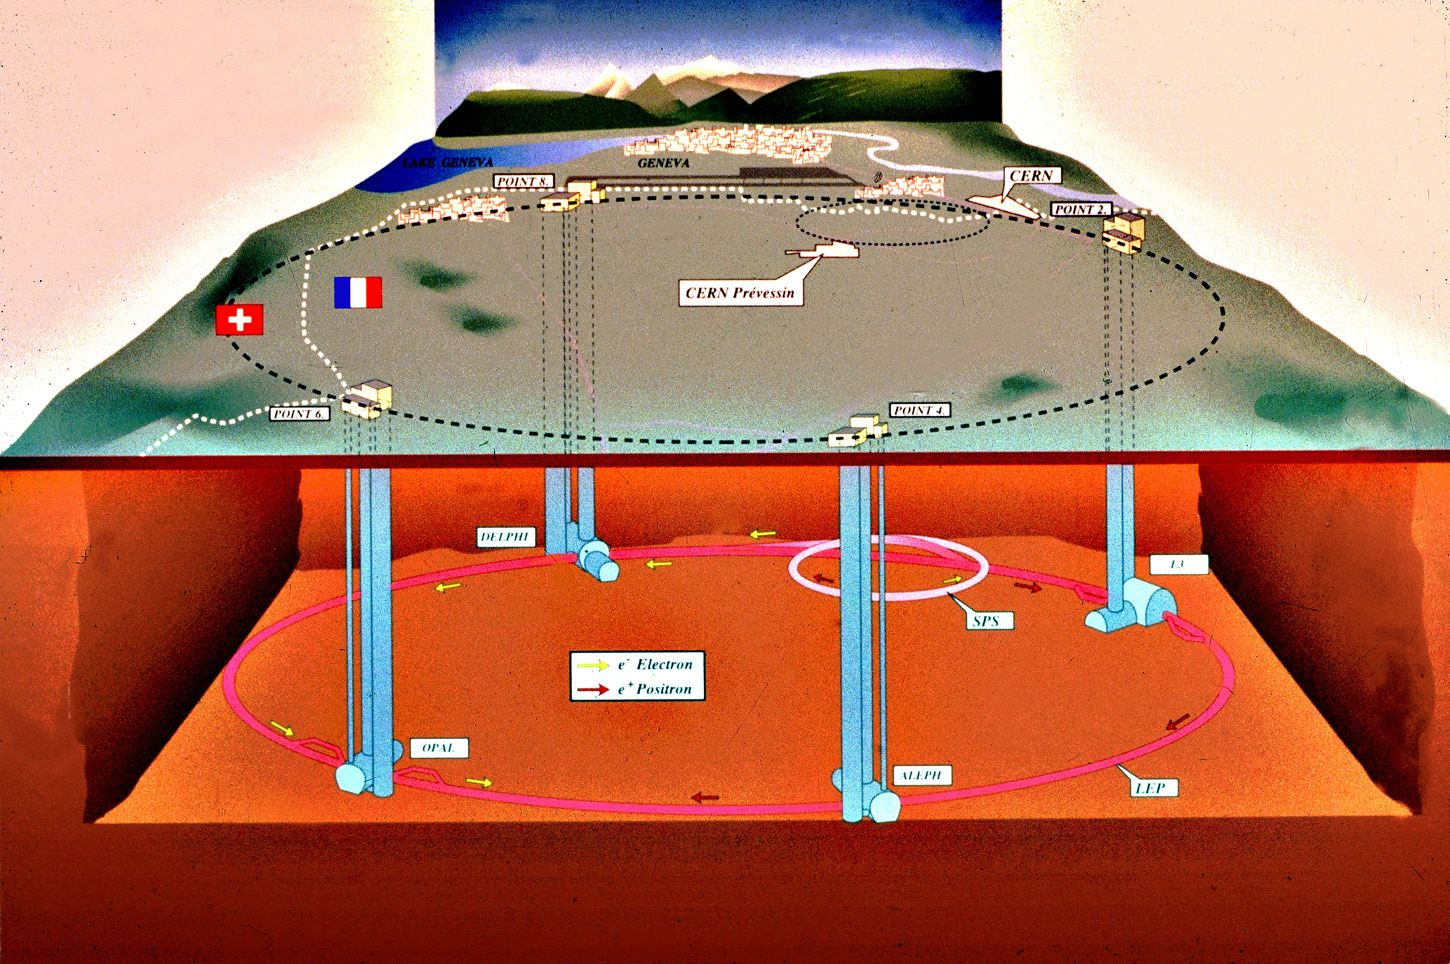
\includegraphics[width=0.8\textwidth]{images/LEP_schema.jpg}
%\caption{}
%\label{fig:example2}
\end{center}
\end{figure}

\small{4 Experiments, each with 400-500 people. Similar experiments were happening at Fermilab, SLAC (Stanford), BNL, DESY (Hamburg), KEK (Tsukuba)...}

\end{frame}



%\begin{frame}
\frametitle{Careers and HEP Sociology in the LHC era}

\begin{itemize}
\item Before the LHC-era particle physicists would typically work on multiple experiments (with different configurations of people) in their career
\item Significant career incentives exist for people to stay within one of these experiments
\item Many examples over the past 10 years of career paths (grad to postdoc to faculty/staff) happen within one LHC experiment
\item J.Birnholz, {\it When Authorship Isn’t Enough: Lessons from CERN on the Implications of Formal and Informal Credit Attribution Mechanisms in Collaborative Research}, \url{http://dx.doi.org/10.3998/3336451.0011.105}
\end{itemize}

\end{frame}




\begin{frame}
\frametitle{S2I2-HEP (Success-oriented) timeline}

\begin{figure}[htbp]
\begin{center}
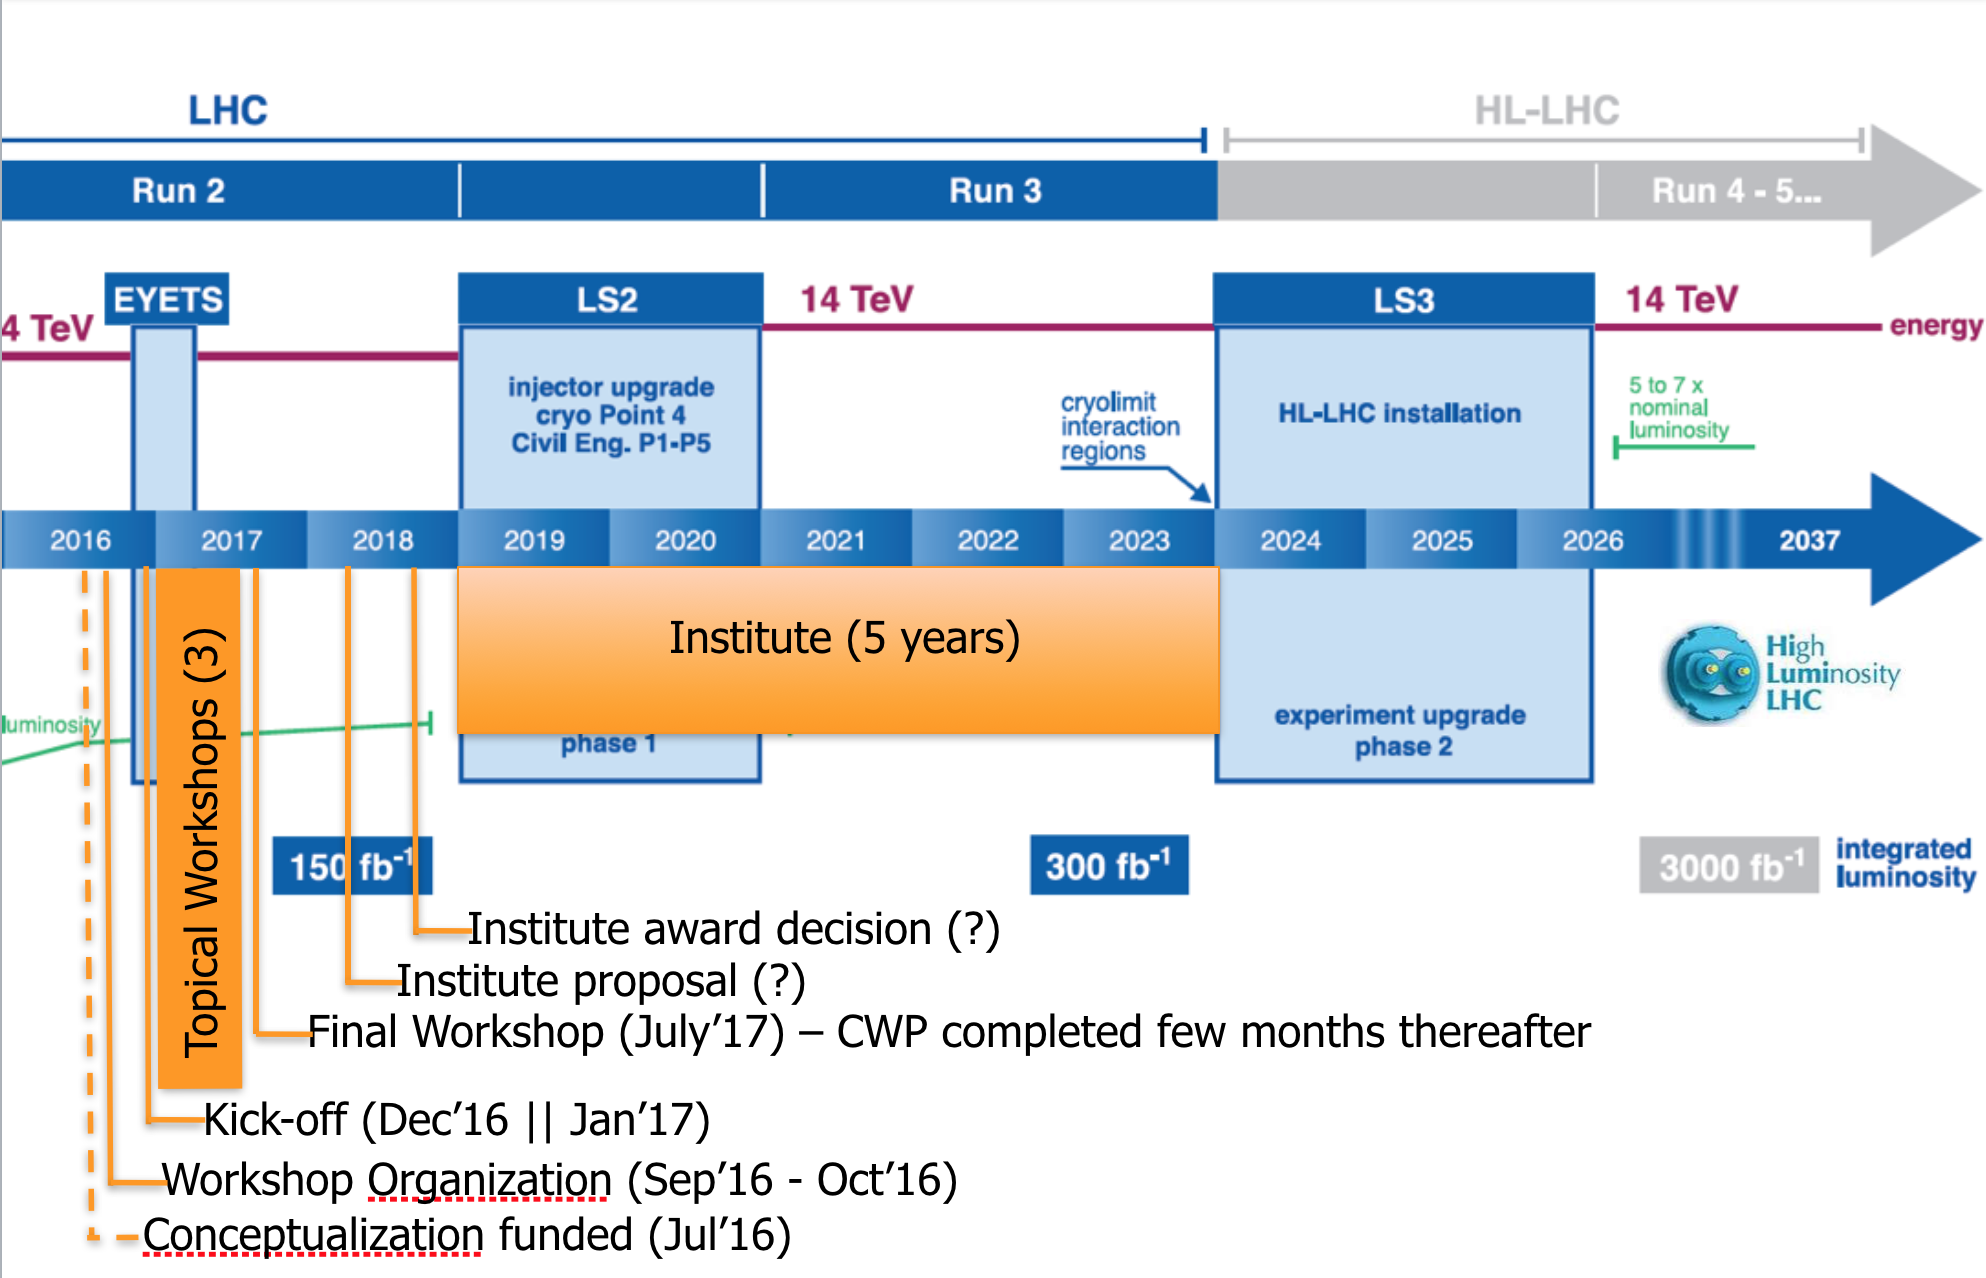
\includegraphics[width=1.0\textwidth]{images/s2i2-hep-timeline.png}
%\caption{}
%\label{fig:example2}
\end{center}
\end{figure}

%\small{Example Text}

\end{frame}



\begin{frame}
\frametitle{Defining Longer-term Strategy}

\begin{itemize}
\item HL-LHC computing requires a major `software upgrade' and an eventual S2I2 institute for HEP would be a major player in that task
\item Planning for such an ``upgrade'' cannot be done for the US (Universities) in isolation
\item Thus we are intiating a larger community process to produce a Community White Paper (CWP) with an overall consensus strategy and roadmap for software and computing in HEP
  \begin{itemize}
  \item Initiated as WLCG charge to the LHC experiments and HSF as a step towards the LHC experiment TDRs in advance of HL-LHC
  \item The scope should not be restricted only to HL-LHC
  \item Some early software components could be built, tested and used by experiments in LHC Run3
  \end{itemize}
\item Organised by the HEP Software Foundation (HSF) [next slide]
\item Paper to be delivered by Summer 2017
\item The S2I2-HEP Strategic Plan will be derived from this global plan
\end{itemize}

\end{frame}



\begin{frame}
\frametitle{HEP Software Foundation (HSF)}

\begin{columns}[T] % align columns

\begin{column}{.75\textwidth}
The HSF (http://hepsoftwarefoundation.org) was created in early 2015 as a means for organizing our community to address the software challenges of future projects such as the HL-HLC. The HSF has the following objectives: 
\end{column}%

\hfill%

\begin{column}{.20\textwidth}
\begin{figure}[htbp]
\begin{center}

\includegraphics[width=1.0\textwidth]{images/hsf_logo_angled.png}
\end{center}
\end{figure}
\end{column}%

\end{columns}

\vskip 0.1in

\begin{itemize}
\item Catalyze new common projects
\item Promote commonality and collaboration in new developments to make the most of limited resources
\item Provide a framework for attracting effort and support to S\&C common projects (new resources!)
\item Provide a structure to set priorities and goals for the work
\end{itemize}

%An initial set of collaborative activities have begun (see recent HSF workshop 
%at LAL-Orsay). 


\end{frame}



\begin{frame}
\frametitle{Community White Paper (CWP)}

\begin{itemize}
\item The CWP will identify and prioritise the software research and development investments required:
   \begin{itemize} 
   \item to achieve improvements in software efficiency, scalability and performance and to make use of the advances in CPU, storage and network technologies
   \item to enable new approaches to computing and software that could radically extend the physics reach of the detectors
   \item to ensure the long term sustainability of the software through the lifetime of the HL-LHC
   \end{itemize} 
\vskip 0.15in
\item The HSF is engaging the HEP community to produce the CWP via a ``community process''
   \begin{itemize} 
   \item Initiated as an HL-LHC planning process
   \item Aiming for a broader participation (LHC, neutrino program, Belle II, linear collider so far)
   \end{itemize} 
\end{itemize}

\end{frame}





%\begin{frame}
\frametitle{Questions from 1st HEP/CS Workshop at NCSA/UIUC}

\footnotesize{
\begin{itemize}
\item What are examples of successful CS-HEP collaborations, and what properties have driven their success?
\item How to align the CS research mechanisms (3 year grants, student developers, conference pubs) with the longer term needs of big science (30 year projects, production software, journal publications)?
\item How to engage a broader slice of the CS community and make scientific computing more “respectable” within CS circles?  (A commonly heard complaint in CS: scientific computing is a ```niche'' research area.)
\item What CS technologies, techniques, and trends could the HEP community adopt, rather than doing everything internally?  (Keeping in mind the long time scales and production needs of HEP.)
\item How could an HEP software institute facilitate interactions between the CS and HEP communities? 
\item What are the incentives for such collaboration for HEP people?  For CS people?  For non-CS people?  E.g. recognition, funding, publications, students, new problems to solve, new places to apply technologies, new solutions to current problems, pride in working on a global-scale problem
\end{itemize}
}

\end{frame}



\begin{frame}
\frametitle{Goals for this workshop}

In the next talk Mark Neubauer will review the discussions we had in the 1st S2I2 HEP/CS workshop at NCSA/UIUC. In this workshop we would like to focus more on possible research collaborations in specific areas:
\begin{itemize}
\item Science Practices \& Policies, Sociology and Community Issues
\item Machine Learning and Algorithms
\item Software Life Cycle / Software Engineering
\item Data Management, Access and Organisation / Data Streaming
\item Data Intensive Analysis Tools, Visualization
\item Scalable Platforms
\item Software/Data/Workflow Preservation \& Reproducibility
\item Training, Education, Professional Development, Advancement
\end{itemize}
\end{frame}



\begin{frame}
\frametitle{Goals for this workshop}
Although the general goal is to identify topics for possible HEP/CS research collaborations, we would like to call out some specific points in that direction:
\begin{itemize}
\item Are there places where the HEP language to describe a problem or system doesn't match how a CS person would describe the same problem?
\item Which things does the HEP community want to do, does not know how, and believes that Computer Scientists may be able to figure out?
\item How do these problems map to CS research questions?
\item Are there CS workshops/meetings on these questions which HEP people should consider attending?
\end{itemize}

\end{frame}




%\begin{frame}
\frametitle{Derived Plans and Proposals} 
The CWP should be the document from which specific plans/proposals can be derived. The US NSF, for example, has indicated a possible path forward to real resources (next slide) to fund a part of such an upgrade project. In parallel to the CWP process proposed here we will prepare a ``Strategic Plan'' for the NSF.
\vskip 0.15in
It should also provide a better context for engaging computer scientists, other sciences and industry (e.g. through CERN Openlab)
\vskip 0.15in
As a community we should be pursuing and preparing the ground for these opportunities in parallel to the preparation of the CWP.
\end{frame}




%\begin{frame}
\frametitle{Detector Simulation, Triggering, Event Reconstruction and Visualization} 
\scriptsize{
Challenges surrounding high pile-up simulation,
including the CPU resources needed for large statistics samples
needed to compare with data from high trigger rates, high memory
utilization, generation and handling of the large (min-bias) samples
needed to achieve accurate description of high pile-up collision
events, and a flexible simulation strategy capable of a broad
spectrum of precision in the detector response, from ``fast''
(e.g. parametric) simulation optimized for speed to full simulation
in support of precision measurements and new physics searches
(e.g. in subtle effects on event kinematics due to the presence of
virtual particles at high scale).
Software required to emulate upgraded detectors (including the
trigger system) and support determination of their optimal
configuration and calibration. $\bullet$
Software in support of triggering
during the HL-LHC, including algorithms for the High-level Trigger,
online tracking using GPUs and/or FPGAs, trigger steering, event
building, data ``parking'' (for offline trigger decision), and data
flow control systems. $\bullet$ New approaches to event reconstruction, in
which the processing time depends sensitively on instantaneous
luminosity, including advanced algorithms, vectorization, and
execution concurrency and frameworks that exploit many-core
architectures. In particular, charged particle tracking is expected
to dominate the event processing time under high pile-up
conditions. $\bullet$ Visualization tools, not only in support of upgrade
detector configurations and event displays, but also as a research
tool for data analysis, education, and outreach using modern tools
and technologies for 3D rendering, data and geometry description and
cloud environments.
}
\end{frame}



%\begin{frame}
\frametitle{Data Access and Management, Workflow and
Resource Management}
\scriptsize{ 
Data handling systems that scale to the Exabyte level during the
HL-LHC era and satisfy the needs of physicists in terms of metadata
and data access, distribution, and replication. Increasing
availability of very high speed networks removes the need for CPU
and data co-location and allows for more extensive use of data
access over the wide-area network (WAN), providing failover
capabilities, global data namespaces, and caching. $\bullet$ Event-based data
streaming as complementary to the more traditional dataset-based or
file-based data access, which is particularly important for
utilizing opportunistic cycles on HPCs, cloud resources, and campus
clusters where job eviction is frequent and stochastic. $\bullet$ Workflow
management systems capable of handling millions of jobs running on a
large number of heterogeneous, distributed computing resources, with
capabilities including whole-node scheduling, checkpointing, job
rebrokering, and volunteer computing. $\bullet$ Systems for measurement and
monitoring of the networking bandwidth and latency between resource
targets and the use of this information in job
brokering. $\bullet$ Software-defined networking technologies which enable
networks to be configurable and schedulable resources for use in the
movement of data.
}

\end{frame}



%\begin{frame}
\frametitle{ Physics generators, Data Analysis and Interpretation, Data and Software Preservation}
\scriptsize{ 
There are many theory challenges in the HL-LHC era, among them are
improving the precision of SM calculations, better estimation of
systematic uncertainties, and elucidation of promising new physics
signals for the experiments. Software needed to make connection
between observations and theory include matrix element generators,
calculation of higher-order QCD corrections, electroweak
corrections, parton shower modeling, parton matching schemes, and
soft gluon resummation methods. Physics generators that employ
concurrency and exploit many-core architectures will play an
important role in HL-LHC, as well better sharing of code and
processing between LHC experimenters and phenomenologists. $\bullet$ Data
analysis frameworks that include parallelization, optimized event
I/O, data caching, and WAN-based data access. Analysis software
that employs advanced algorithms and efficiently utilizes many-core
architectures. $\bullet$ Tools and technologies for preservation and reuse of
data and software, preservation and re-interpretation of physics
results, analysis providence and workflow ontologies, analysis
capture, and application packaging for platform abstraction. $\bullet$ Future
software repositories and build platforms that leverage advances in
these areas and improved software modularity and quality control
that will allow a broader community of people to effectively
contribute to software in the HL-LHC era.}

\end{frame}



%\begin{frame}
\frametitle{Community Roadmap Process}

We propose a series of workshops over the next year to build the community roadmap:

\begin{itemize}
\item Initial presentation and organization this month (at WLCG workshop and CHEP, etc.)
  \begin{itemize}
  \item Flesh out the charges and attract interested individuals to the WGs
  \end{itemize}
\item A ``kick-off'' workshop at UC San Diego on 23-26 Jan 2017
  \begin{itemize}
  \item Start real work after a few months post-CHEP gestation in the WGs
  \item Discussions on more controversial topics, find path to consensus
  \item Develop plans and responsibilities for delivering white paper by summer 2017
  \end{itemize}
\item Possible ``topical'' workshops between Jan-Jun 2017, building on existing community activities when possible (e.g.\ DPHEP, Reco Algorithms Forum/CTD, IML)
\item A final workshop in summer 2017 (in Europe, near CERN?)
\end{itemize}

\end{frame}



%\begin{frame}
\frametitle{Practicalities: CWP Process}

\begin{itemize}
\item The end goal here is a single (consensus) CWP roadmap for the community. 
\item Finding consensus in a large community is a difficult task: broad participation and visibility/transparency are key elements
\item The process being used largely mirrors that used in the ``decadal survey'' process in high energy physics
\item Working groups self-organize, with encouragement from institutions and projects/experiments/etc.
\item A series of workshops is planned over about 9 months to allow topics to be explored, sometimes overloading CWP discussions onto preexisting meetingd
\item Contributions along the way can come in the form of ``white papers'' by individuals/groups/projects/institutions
\item Based on the ideas emerging from the discusions, workshops and white papers, a consensus CWP document will be written.
\end{itemize}

\end{frame}



%\begin{frame}
\frametitle{Practicalities: Possible Working Groups}
\begin{table}[h!]
\tiny
\centering
\label{tab:table1}
\begin{tabular}{|l|l|}
\hline
Detector Simulation & full and fast simulations, hi-pileup environments \\ \hline

Triggering & algorithms, GPUs and/or FPGAs \\ \hline

Event Reconstruction & new approaches to event reconstruction \\ \hline

Visualization & tools for data analysis, education, and outreach \\ \hline

Data Access and Management & scaling to the exabyte level \\ \hline

Workflow and Resource Management & millions of jobs in heterogenous systems \\ \hline

Physics generators & better models, better precision, code optimisations \\ \hline

Data Analysis and Interpretation & efficient use of many-core, modern techniques \\ \hline

Data and Software Preservation & preservation and reuse of data and software \\ \hline

Software Development, Deployment & \\
and Validation/Verification & improved modularity and quality, contribution \\ \hline

Computing Models, Facilities, & \\
Distributed Computing & range of possible models, costing\\ \hline

Various Aspects of Technical Evolution & \\ 
(Software Tools, Hardware) &  \\ \hline

Security and Access Control & \\ \hline

Careers, Staffing and Training & perhaps in a separate concurrent white paper \\ \hline

Machine Learning & \\ \hline

Conditions Database & \\ \hline

Event Processing Frameworks & \\ \hline
\end{tabular}
\end{table}

\begin{center}
\small{More details in links at \color{blue} {\url{http://hepsoftwarefoundation.org/cwp.html}}}
\end{center}

\end{frame}



%\begin{frame}
\frametitle{HSF Community White Paper Workshop at SDSC}

\begin{itemize}
\item The kick-off workshop for the HSF CWP process will be on 23-26 January 2017 at SDSC/UCSD
\item \url{http://indico.cern.ch/event/570249/}
\item People from many HEP experiments (LHC and beyond)
\item A key element in the ``community process'' to form a consensus
\item We are looking for opportunities to introduce new ideas into the HEP discussions
\item Additional topical workshops will happen in the spring and a final workshop (``near CERN'' in summer 2017) is planned
\item Further information about these will be posted on the s2i2-hep google group and at \url{http://s2i2-hep.org}
\end{itemize}

\end{frame}






%\begin{frame}
\frametitle{Summary}

\begin{itemize}
\item Questions?
\end{itemize}



\end{frame}




\end{document}


